\documentclass[12pt,oneside,a4paper,PisaPhdThesis, italian]{PhdThesis}
\usepackage[centertags]{amsmath}
\usepackage{framed}
\usepackage{libertine}
\usepackage{csquotes}
\usepackage[italian, english]{babel}
\usepackage[font=small,labelfont=bf,tableposition=top]{caption}
\usepackage{graphics}
\usepackage{graphicx}
\usepackage{wrapfig}
\usepackage{color}
\usepackage{hyperref}
\usepackage{epsfig}
\usepackage{amsfonts}
\usepackage{amssymb}
\usepackage{amsthm}
\usepackage{rawfonts}
\usepackage{enumerate}
\usepackage{enumitem}
\usepackage{capt-of}
\usepackage{url}
\usepackage{xspace}
\usepackage{xthesis} 
\usepackage{xtocinc}
\usepackage{listings}    
\usepackage{courier}
\usepackage[dvipsnames]{xcolor}
%Necessari per blocchi di codice
\definecolor{commentgreen}{rgb}{0,0.45,0}
\definecolor{codepurple}{rgb}{0.58,0,0.82}
\definecolor{backcolour}{rgb}{0.95,0.95,0.92}
\definecolor{darkred}{rgb}{0.6,0.0,0.0}
\definecolor{lightblue}{rgb}{0.0,0.42,0.91}
\colorlet{punct}{red!60!black}
\definecolor{delim}{RGB}{20,105,176}
\colorlet{numb}{magenta!60!black}
\lstdefinelanguage{json}{
	keywords=[1]{items, type, properties, const, name, checks, $schema, check_type, required, operator, operand_, minItems, uniqueItems, state_names, parent_names, enum_names, event_names, fn_names, callable_function, parameters_list, storage_location, modifiers, binary_operations, anyOf, nome, cognome, genere, via, indirizzo, eta, citta, paese, interessi, Ownable, AccessRestriction, AutoDeprecation, BalanceLimit, CheckEffectsInteraction, CircuitBreaker, CommitReveal, EternalStorage, GuardCheck, MemoryArrayBuilding, Mortal, Mutex, Oracle, Ownership, PullOverPush, Randomness, RateLimit, Rejector, Relay, SecureTransfer, StateMachine, StringEquality, TightVariablePacking},
	keywordstyle=\color{codepurple}\bfseries,
	keywords=[2]{true, false},
	keywordstyle=[2]\color{lightblue}\bfseries,
	literate=
	*{0}{{{\color{numb}0}}}{1}
	{1}{{{\color{numb}1}}}{1}
	{2}{{{\color{numb}2}}}{1}
	{3}{{{\color{numb}3}}}{1}
	{4}{{{\color{numb}4}}}{1}
	{5}{{{\color{numb}5}}}{1}
	{6}{{{\color{numb}6}}}{1}
	{7}{{{\color{numb}7}}}{1}
	{8}{{{\color{numb}8}}}{1}
	{9}{{{\color{numb}9}}}{1}
	{:}{{{\color{punct}{:}}}}{1}
	{,}{{{\color{punct}{,}}}}{1}
	{\{}{{{\color{delim}{\{}}}}{1}
	{\}}{{{\color{delim}{\}}}}}{1}
	{[}{{{\color{delim}{[}}}}{1}
	{]}{{{\color{delim}{]}}}}{1},
}

\lstdefinelanguage{Solidity}{
	keywords=[1]{anonymous, assembly, assert, balance, break, call, callcode, case, catch, class, constant, continue, constructor, contract, debugger, default, delegatecall, delete, do, else, emit, event, experimental, export, external, false, finally, for, function, gas, if, implements, import, in, indexed, instanceof, interface, internal, is, length, library, log0, log1, log2, log3, log4, memory, modifier, new, payable, pragma, private, protected, public, pure, push, require, return, returns, revert, selfdestruct, send, solidity, storage, struct, suicide, super, switch, then, this, throw, transfer, true, try, typeof, using, value, view, while, with, addmod, ecrecover, keccak256, mulmod, ripemd160, sha256, sha3, virtual, override, abstract}, % generic keywords including crypto operations
	keywordstyle=\color{codepurple}\bfseries,
	keywords=[2]{address, bool, byte, bytes, bytes1, bytes2, bytes3, bytes4, bytes5, bytes6, bytes7, bytes8, bytes9, bytes10, bytes11, bytes12, bytes13, bytes14, bytes15, bytes16, bytes17, bytes18, bytes19, bytes20, bytes21, bytes22, bytes23, bytes24, bytes25, bytes26, bytes27, bytes28, bytes29, bytes30, bytes31, bytes32, enum, int, int8, int16, int24, int32, int40, int48, int56, int64, int72, int80, int88, int96, int104, int112, int120, int128, int136, int144, int152, int160, int168, int176, int184, int192, int200, int208, int216, int224, int232, int240, int248, int256, mapping, string, uint, uint8, uint16, uint24, uint32, uint40, uint48, uint56, uint64, uint72, uint80, uint88, uint96, uint104, uint112, uint120, uint128, uint136, uint144, uint152, uint160, uint168, uint176, uint184, uint192, uint200, uint208, uint216, uint224, uint232, uint240, uint248, uint256, var, void, ether, finney, szabo, wei, days, hours, minutes, seconds, weeks, years},	% types; money and time units
	keywordstyle=[2]\color{teal}\bfseries,
	keywords=[3]{block, blockhash, coinbase, difficulty, gaslimit, number, timestamp, msg, data, gas, sender, sig, value, now, tx, gasprice, origin},	% environment variables
	keywordstyle=[3]\color{lightblue}\bfseries,
	sensitive=true,
	comment=[l]{//},
	morecomment=[s]{/*}{*/},
	morestring=[b]',
	morestring=[b]"
}

\lstset{
	frame=lines,
	backgroundcolor=\color{backcolour},
	basicstyle=\scriptsize\ttfamily,
	breakatwhitespace=false,         
	breaklines=true,                 
	captionpos=b,                    
	keepspaces=true,                 
	numbers=left,  
	numberstyle=\tiny,                 
	numbersep=5pt,                  
	showspaces=false,                
	showstringspaces=false,
	showtabs=false,                  
	tabsize=2,
	framextopmargin=3pt,
	framexbottommargin=3pt,
	framexleftmargin=3pt,
	commentstyle=\color{commentgreen}\ttfamily,
	keywordstyle=\color{blue}\bfseries,
	identifierstyle=\color{black}\ttfamily,
	stringstyle=\color{darkred}\ttfamily,
}
\addto\captionsitalian{%
	\renewcommand{\lstlistingname}{Codice}}
%END - Necessari per blocchi di codice

%per grafici
\usepackage{float}
\usepackage{tikz}
\usepackage{pgfplots} 
\pgfplotsset{compat=1.16} 
\usetikzlibrary{datavisualization}
%END - Per grafici

\newlength{\defbaselineskip}
\setlength{\defbaselineskip}{\baselineskip}
\newcommand{\setlinespacing}[1]%
           {\setlength{\baselineskip}{#1 \defbaselineskip}}
\newcommand{\doublespacing}{\setlength{\baselineskip} {2.0 \defbaselineskip}}
\newcommand{\singlespacing}{\setlength{\baselineskip}{\defbaselineskip}}
\newcommand{\mycenterline}[1]{\vspace{.1cm}\newline\vspace{.1cm}\centerline{#1}}

% Bibliografia
\usepackage[sorting=none]{biblatex}
\addbibresource{components/bibliografica.bib}
%END - Bibliografia


\begin{document}
\selectlanguage{italian}
\graphicspath{ {./components/images/} }
\begin{titlepage}
	
\centering


\includegraphics[scale=0.25]{components/images/university-logo}

\bigskip

\gdef\@phd@university{
	{\LARGE \bfseries Universit\`{a} degli Studi di Catania}\\ 
	{\large Dipartimento di Matematica e Informatica}\\ 
	{Corso di Laurea Triennale in Informatica}\\
	\bigskip}

\textsc{\@phd@university}\par

\hrule

\bigskip

\bigskip

\bigskip

\bigskip

\bigskip

\bigskip

{\itshape \large
	Alessio Tudisco\par
}

\bigskip

\bigskip

\bigskip

\bigskip

\bigskip

\bigskip

{\Large Analisi Statica Solidity: Ricerca Design Pattern}\par

\bigskip

\bigskip

\bigskip

\bigskip

\bigskip

\bigskip

\begin{minipage}[b]{8 cm}
	\hrule
	
	\bigskip
	
	{\centering \scshape Relazione Progetto Finale\par}
	
	\bigskip
	
	\hrule
\end{minipage}

\bigskip

\bigskip

\bigskip

\bigskip

\bigskip

\bigskip

\begin{tabular}[t]{ccc}
	
	\textsc{} & \hspace{8cm} &\textsc{Relatore}\\
	& \hspace{8cm} & Prof. Emiliano Alessio Tramontana\\
	
\end{tabular}

\bigskip

\begin{tabular}[t]{ccc}
	
	\textsc{} & \hspace{8cm} &\textsc{Correlatore}\\
	& \hspace{8cm} & /\\
	
\end{tabular}

\bigskip

\bigskip

\bigskip

\bigskip

\bigskip

\bigskip

\bigskip

\bigskip

\bigskip

\bigskip

\bigskip

\hrule

\bigskip

{
	Anno Accademico 2021 - 2022\par
}
\end{titlepage}


\chaptertitlestyle{serifbig}
\pagestyle{serif}
\setlinespacing{1.15}
\chapter*{Abstract}\label{abstract}
Blockchain technologies assume a key role in Web3, the next generation of the World Wide Web, whose goal is to create a decentralized and autonomous Internet in which users have greater control and ownership of their online data and activities. Within Ethereum blockchain, automated digital contracts, called \textit{smart-contracts}, are executed when certain conditions are met. Smart-contracts are written in code by a developer and as such are susceptible to vulnerabilities and security problems. A coding error or vulnerability can allow an attacker to compromise the contract and cause extensive and irreparable damage. Therefore, it is important that smart-contracts are carefully written and tested to ensure that they are free of vulnerabilities and function as intended.\\
\\
The goal of this thesis is to study, analyze, automating the process, and report which and \textit{design patterns} are currently used in the development of Ethereum blockchain smart-contracts.
\vspace{40pt}
\begin{center}
\large$\star\star\star$
\end{center}
\vspace{40pt}
Le tecnologie blockchain assumono un ruolo chiave nel Web3, la prossima generazione del World Wide Web, il cui obiettivo è creare un Internet decentralizzato e autonomo in cui gli utenti hanno maggiore controllo e proprietà dei propri dati e attività online. All'interno della blockchain Ethereum vengono eseguiti, quando determinate condizioni sono soddisfatte, dei contratti digitali automatizzati, denominati \textit{smart-contract}. Gli smart-contract sono scritti in codice da un programmatore e come tali sono suscettibili a vulnerabilità e problemi di sicurezza. Un errore di codifica o una vulnerabilità può permettere a un attaccante di compromettere il contratto e causare danni ingenti e irreparabili. Pertanto, è importante che gli smart-contract vengano scritti e testati con cura per garantire che siano privi di vulnerabilità e funzionino come previsto.\\
\\
L'obiettivo di questa tesi è studiare, analizzare, automatizzando il processo, e documentare quali \textit{design pattern} siano attualmente utilizzati nello sviluppo degli smart-contract della blockchain Ethereum.
 


\begin{frontmatter}
\setlinespacing{1.1}
\pagenumbering{Roman}
\addtocontents{toc}{\protect\setcounter{tocdepth}{-1}}
\tableofcontents
\addtocontents{toc}{\protect\setcounter{tocdepth}{3}}
\end{frontmatter}

\begin{frontmatter}\end{frontmatter}

\pagenumbering{arabic}
\chapter{Introduzione e Contesto}
L'attuale generazione della tecnologia World Wide Web, denominata \textit{Web2}, è caratterizzata da una maggiore interattività e partecipazione degli utenti rispetto alla precedente generazione, detta \textit{Web1}. In genere, con il termine Web2, si denota la transizione dalla semplice navigazione di siti web all'utilizzo, da parte degli utenti della rete, di servizi e applicazioni interattive, come ad esempio: i social network, le piattaforme di streaming e gli e-commerce.

Questa seconda generazione è anche caratterizzata da un \textit{problema di centralizzazione}, il quale consiste nel fatto che molte delle informazioni e dei dati che circolano in rete sono gestiti da un numero ristretto di grandi aziende. Ciò può portare a problemi di privacy, sicurezza e libertà d'espressione, in quanto queste aziende possono utilizzare i dati degli utenti per fini commerciali o per influenzare l'accesso a determinate informazioni. Inoltre, la centralizzazione introduce problemi di dipendenza e vulnerabilità, in quanto un'unica entità ha il controllo sui dati e sui servizi forniti, la quale, se attaccata attraverso vulnerabilità, può essere soggetta al furto di una grande mole di dati sensibili.

La prossima generazione, denominata \textit{Web3}, punta a risolvere questo problema attraverso la decentralizzazione e la creazione di applicazioni e servizi che non dipendono da un'unica entità o autorità centrale, ma che sono gestiti da una rete di nodi distribuiti. In questo modo, si mira a creare una rete più equa, sicura e resiliente, dove gli utenti hanno il controllo dei propri dati e delle proprie informazioni.

Di seguito in questo capitolo vengono presentati i concetti fondamentali del Web3, il tema d'interesse della tesi, le modalità e il lavoro svolto per lo svolgimento quest'ultimo e la struttura generale della tesi.
\section{Le blockchain}
Le blockchain sono una tecnologia di registro distribuito che consente la creazione di una rete peer-to-peer senza la necessità di intermediari. Ciò significa che le transazioni e le informazioni possono essere scambiate direttamente tra gli utenti senza la necessità di un'autorità centrale. Ciò rende le blockchain adatte per la creazione di un Internet decentralizzato in cui gli utenti hanno maggiore sicurezza, trasparenza e autonomia.\\
Gli smart contract sono una forma di contratto digitale automatizzato che si esegue automaticamente quando determinate condizioni sono soddisfatte. Essi sono scritti in un linguaggio di programmazione che consente la creazione di regole e logiche specifiche che vengono eseguite su una blockchain.

Gli smart contract consentono la creazione di accordi automatici tra le parti in modo da ridurre i tempi di elaborazione e i costi associati alle transazioni tradizionali. Inoltre, essi possono essere utilizzati per creare applicazioni decentralizzate (dApps) che utilizzano la tecnologia blockchain per garantire la sicurezza e la trasparenza delle transazioni.

Per quanto riguarda la sicurezza, gli smart contract sono scritti in codice e come tali sono suscettibili a vulnerabilità e problemi di sicurezza. Un errore di codifica o una vulnerabilità può permettere a un attaccante di compromettere il contratto e causare danni irreparabili. Pertanto, è importante che gli smart contract vengano scritti e testati con cura per garantire che siano privi di vulnerabilità e funzionino come previsto.

\section{Struttura Tesi}
Di seguito vengono illustrati gli argomenti trattati in ogni capitolo presente:
\begin{itemize}
	\item Nel \textit{capitolo 2} vengono introdotti gli strumenti utilizzati per lo svolgimento del tema della tesi;
	\item Nel \textit{capitolo 3} vengono descritti i design pattern individuati nello studio dell'attuale divulgazione scientifica;
	\item Nel \textit{capitolo 4} viene presentato il software di analisi statica automatica sviluppato;
	\item Nel \textit{capitolo 5} vengono riportati i risultati dell'analisi automatica di alcuni smart-contract open-source;
	\item Nell'\textit{appendice} vengono riportati i codici di riferimento dei design pattern usati per lo sviluppo del software;
\end{itemize}
\chapter{Strumenti Utilizzati}
I design pattern adottati nello sviluppo di smart-contract possono essere classificati in diversi tipi\cite[alcuni tipi]{9089272}\cite{9050163}, ognuno dei quali caratterizza un aspetto specifico della lifecycle del contratto:

\begin{itemize}
	\item \textit{Authorization}: relativi alla gestione dell'accesso alle funzionalità del contratto;
	\item \textit{Behavioral}: relativi a meccanismi di supporto per il corretto svolgimento delle funzionalità del contratto;
	\item \textit{Gas Economic}: relativi a meccanismi per ridurre il consumo di \textit{gas} durante l'esecuzione delle funzionalità del contratto;
	\item \textit{Lifecycle}: relativi alla a meccanismi per la creazione e la distruzione del contratto;
	\item \textit{Maintenance}: relativi a meccanismi di supporto per la manutenzione del contratto;
	\item \textit{Security}: relativi a meccanismi per la mitigazione di vulnerabilità di sicurezza note;
\end{itemize}

\section{Authorization Design Pattern}
La blockchain di Ethereum non implementa meccanismi di autenticazione o di ruoli/permessi per consentire l'accesso alle funzionalità di un contratto solo nel caso in cui vengano soddisfatte determinate condizioni. Per la natura della blockchain, ogni funzione definita con visibilità pubblica può essere invocata da qualsiasi utente.\par
Gli \textit{Authorization Design Pattern} offrono meccanismi atti a limitare l'esecuzione delle funzionalità di un contratto. Si individuano i seguenti design pattern: \textit{Ownership} e \textit{Access Restriction}.
\subsection{Ownership Pattern}
L’\textit{Ownership} pattern offre un meccanismo per riservare al proprietario di uno smart-contract l’esecuzione di funzionalità critiche, a cui l’utente finale non deve avere accesso.\par
Opzionalmente possono essere implementati anche meccanismi di supporto per eseguire l’operazione di trasferimento del titolo di proprietario.
\begin{table}[H]\label{Ownership_table}
	\caption{Specifiche dell'Ownership Pattern}
	\centering
	\begin{tikzpicture}
		\node (table) [inner sep=0pt] {
			\def\arraystretch{1.5}
			\begin{tabular}{p{0.30\linewidth} | p{0.65\linewidth}}
				\textbf{Problema} & {Nella blockchain di Ethereum, qualsiasi utente può richiamare qualunque funzione, definita con visibilità pubblica, di un contratto, ma in certi use-case potrebbe essere necessario riservare l’esecuzione di specifiche funzioni al solo proprietario.} \\ \hline
				\textbf{Soluzione} & {Memorizzare in una variabile di stato del contratto l'indirizzo del proprietario e limitare l'esecuzione delle funzioni in base all'indirizzo del chiamante.} \\ \hline
				\textbf{Riconoscimento} & {Individuare un confronto fra \textit{msg.sender} e la variabile di stato contenente l’indirizzo del proprietario.\par Il confronto può essere implementato attraverso un \textit{modifier} o la funzione \textit\mbox{\textit{require()}}.} \\ \hline
				\textbf{Snippet di Codice\newline(Versione Semplificata)} & Il codice sorgente di riferimento è consultabile nell'appendice: \ref{appendix:ownership}  \\ \hline
				\textbf{Riferimenti} & \cite[Ownership]{maxwoe} \cite[Ownership]{cjgdev} \cite[Access Restriction]{fravoll} \\
			\end{tabular}
		};
		\draw [rounded corners=.5em] (table.north west) rectangle (table.south east);
	\end{tikzpicture}
\end{table}
\newpage
\subsection{Access Restriction Pattern}
L’\textit{Ownership} pattern offre un meccanismo per riservare al proprietario di uno smart-contract l’esecuzione di funzionalità critiche, a cui l’utente finale non deve avere accesso.\par
Opzionalmente possono essere implementati anche meccanismi di supporto per eseguire l’operazione di trasferimento del titolo di proprietario.
\begin{table}[H]\label{Access_Restriction_table}
	\caption{Specifiche dell'Ownership Pattern}
	\centering
	\begin{tikzpicture}
		\node (table) [inner sep=0pt] {
			\def\arraystretch{1.5}
			\begin{tabular}{p{0.30\linewidth} | p{0.65\linewidth}}
				\textbf{Problema} & {Nella blockchain di Ethereum, qualsiasi utente può richiamare qualunque funzione, definita con visibilità pubblica, di un contratto, ma in certi use-case potrebbe essere necessario riservare l’esecuzione di specifiche funzioni al solo proprietario.} \\ \hline
				\textbf{Soluzione} & {Memorizzare in una variabile di stato del contratto l'indirizzo del proprietario e limitare l'esecuzione delle funzioni in base all'indirizzo del chiamante.} \\ \hline
				\textbf{Riconoscimento} & {Individuare un confronto fra \textit{msg.sender} e la variabile di stato contenente l’indirizzo del proprietario.\par Il confronto può essere implementato attraverso un \textit{modifier} o la funzione \textit\mbox{\textit{require()}}.} \\ \hline
				\textbf{Snippet di Codice\newline(Versione Semplificata)} & 
				You can find the raw data used to calculate this metrics in Appendix \ref{appendix:ownership}.\\ \hline
				\textbf{Riferimenti} & \cite[Ownership]{maxwoe} \cite[Ownership]{cjgdev} \cite[Access Restriction]{fravoll} \\
			\end{tabular}
		};
		\draw [rounded corners=.5em] (table.north west) rectangle (table.south east);
	\end{tikzpicture}
\end{table}
\chapter{Classificazione dei Design Pattern per Smart-Contract}
I design pattern adottati nello sviluppo di smart-contract possono essere classificati in diversi tipi, alcuni descritti in \cite{9089272} e \cite{9050163}, ognuno dei quali caratterizza un aspetto specifico della lifecycle del contratto:

\begin{itemize}
	\item \textit{Authorization}: relativi alla gestione dell'accesso alle funzionalità del contratto;
	\item \textit{Behavioral}: relativi a meccanismi di supporto per il corretto svolgimento delle funzionalità del contratto;
	\item \textit{Gas Economic}: relativi a meccanismi per ridurre il consumo di \textit{gas} durante l'esecuzione delle funzionalità del contratto;
	\item \textit{Lifecycle}: relativi alla a meccanismi per la creazione e la distruzione del contratto;
	\item \textit{Maintenance}: relativi a meccanismi di supporto per la manutenzione del contratto;
	\item \textit{Security}: relativi a meccanismi per la mitigazione di vulnerabilità di sicurezza note;
\end{itemize}
\textit{Essendo Solidity un linguaggio di programmazione tutt'ora in sviluppo, quindi soggetto a cambiamenti, e le pubblicazioni, scientifiche e di programmatori, alquanto datate, tutti i design pattern individuati sono stati aggiornati dal punto di vista sintattico per essere compatibili con la versione 0.8.0.0 o superiore di Solidity}. 
\newpage
{\section{Authorization Design Pattern}
La blockchain Ethereum non implementa meccanismi di autenticazione o di permessi per consentire l'accesso a specifiche funzionalità di un contratto solo nel caso in cui vengano soddisfatte determinate condizioni. Per la natura della blockchain, ogni funzione definita con visibilità pubblica può essere invocata da qualsiasi utente.\par
Gli \textit{Authorization Design Pattern} propongono meccanismi atti a limitare l'esecuzione delle funzionalità di un contratto.\par
Si individuano i seguenti design pattern: \textit{Access Restriction} e \textit{Ownership}.
{\subsection{Access Restriction Pattern}
	L'\textit{Access Restriction} pattern propone un meccanismo per introdurre dei controlli di prerequisiti nella logica del contratto.\par
	Il meccanismo proposto si basa sul concetto di \textit{function modifiers} presente in Solidity, che permette di definire dei controlli che possono essere eseguiti prima o dopo l'esecuzione del corpo della funzione a cui viene applicato il \textit{modifier}.
	\begin{table}[H]
		\centering
		\begin{tikzpicture}
			\node (table) [inner sep=0pt] {
				\def\arraystretch{1.5}
				\begin{tabular}{p{0.21\linewidth} | p{0.74\linewidth}}
					\textbf{Problema} & {Qualsiasi utente può richiamare qualunque funzione definita con visibilità pubblica di un contratto, ma in certi scenari potrebbe essere necessario definire dei prerequisiti o condizioni ed eseguire la funzionalità richiesta solo al verificarsi di essi.} \\ \hline
					\textbf{Soluzione} & {Definire una serie di \textit{modifier} di uso generale, che verifichino i prerequisiti desiderati, e applicarli nella definizione delle funzioni interessate.} \\ \hline
					\textbf{Riconoscimento} & {Individuare,  all'interno del contratto, la definizione o utilizzo di \textit{modifier}.} \\ \hline
					\textbf{Riferimenti} & {Codice di riferimento: \ref{appendix:access_restriction} \newline Bibliografia: \cite{maxwoe} \cite{cjgdev} \cite{fravoll}} \\
				\end{tabular}
			};
			\draw [rounded corners=.5em] (table.north west) rectangle (table.south east);
		\end{tikzpicture}
		\caption{Specifiche dell'Access Restriction Pattern}
	\end{table}
}
\newpage
{\subsection{Ownership Pattern}
L'\textit{Ownership} pattern propone un meccanismo per riservare al proprietario di uno smart-contract l'esecuzione di funzionalità critiche, a cui l'utente finale non deve avere accesso.\par
Opzionalmente, possono essere implementati anche meccanismi di supporto per l'operazione di trasferimento del titolo di proprietario.\par
Questo design pattern può essere considerato come un caso specifico di Access Restriction.
\begin{table}[H]
	\centering
	\begin{tikzpicture}
		\node (table) [inner sep=0pt] {
			\def\arraystretch{1.5}
			\begin{tabular}{p{0.21\linewidth} | p{0.74\linewidth}}
				\textbf{Problema} & {Qualsiasi utente può richiamare qualunque funzione definita con visibilità pubblica di un contratto, ma in certi scenari potrebbe essere necessario riservare l'esecuzione di specifiche funzioni al solo proprietario.} \\ \hline
				\textbf{Soluzione} & {Memorizzare in una variabile di stato del contratto l'indirizzo del proprietario e limitare l'esecuzione delle funzioni in base all'indirizzo del chiamante.} \\ \hline
				\textbf{Riconoscimento} & {Individuare un confronto fra l'indirizzo del chiamante, contenuto in \textit{msg.sender}, e la variabile di stato contenente l'indirizzo del proprietario. Il confronto può essere eseguito attraverso un costrutto \textit{if-else}, \textit{modifier} o la funzione \textit\mbox{\textit{require()}}.} \\ \hline
				\textbf{Riferimenti} & {Codice di riferimento: \ref{appendix:ownership} \newline Bibliografia: \cite{maxwoe} \cite{cjgdev} \cite[Incluso in Access Restriction]{fravoll}} \\
			\end{tabular}
		};
		\draw [rounded corners=.5em] (table.north west) rectangle (table.south east);
	\end{tikzpicture}
	\caption{Specifiche dell'Ownership Pattern}
\end{table}
}
}
\newpage
{\section{Behavioral Design Pattern}
I \textit{Behavioral design pattern} propongono funzionalità e meccanismi di supporto per facilitare lo svolgimento delle operazioni del contratto.\par
Si individuano i seguenti design pattern: \textit{Commit \& Reveal}, \textit{Guard Check}, \textit{Oracle}, \textit{Pull Payment (Pull over Push)}, \textit{Randomness} e \textit{State Machine Pattern}.
{\subsection{Commit and Reveal Pattern}
	Il \textit{Commit and Reveal} pattern propone un meccanismo per consentire agli utenti di uno smart-contract di attenersi a un valore tenendolo nascosto agli altri con la possibilità di rivelarlo in seguito.
	\begin{table}[H]
		\centering
		\begin{tikzpicture}
			\node (table) [inner sep=0pt] {
				\def\arraystretch{1.5}
				\begin{tabular}{p{0.21\linewidth} | p{0.74\linewidth}}
					\textbf{Problema} & {Essendo Ethereum una blockchain pubblica, tutti i dati e tutte le transazioni sono visibili pubblicamente. Si può facilmente immaginare uno scenario, come una scommessa basata sul gioco carta-forbici-sasso, in cui le interazioni con lo smart-contract, particolarmente i valori dei parametri inviati, debbano essere trattate in modo confidenziale.} \\ \hline
					\textbf{Soluzione} & {Implementare uno \textit{schema di commitment}. Uno schema di commitment è un algoritmo crittografico utilizzato per consentire a qualcuno di impegnarsi su un valore tenendolo nascosto ad altri con la possibilità di rivelarlo in seguito. I valori in uno schema di commitment sono vincolanti, ovvero nessuno può cambiarli una volta impegnati. Lo schema prevede due fasi: una fase di \textit{commit}, in cui viene scelto e specificato un valore, e una fase di \textit{reveal}, in cui il valore viene rivelato e utilizzato.} \\ \hline
					\textbf{Riconoscimento} & {Data la complessità e la libertà implementativa, il riconoscimento di questo design pattern si basa sulla ricerca di definizione e uso di funzioni denominate \textit{"commit"} e \textit{"reveal"} e sulla definizione degli eventi \textit{"LogCommit"} e \textit{"LogReveal"}. \textit{Si potrebbe affinare il riconoscimento tentanto di rilevare una struct di commit}.} \\ \hline
					\textbf{Riferimenti} & {Codice di riferimento: \ref{appendix:commit_and_reveal} \newline Bibliografia: \cite{maxwoe}} \\
				\end{tabular}
			};
			\draw [rounded corners=.5em] (table.north west) rectangle (table.south east);
		\end{tikzpicture}
		\caption{Specifiche del Commit and Reveal Pattern}
	\end{table}
}
\newpage
{\subsection{Guard Check}
	Nella blockchain Ethereum non vi sono regolatori o mediatori, ma vi è necessità di controlli per assicurare che lo smart-contract funzioni come previsto.\par
	Il \textit{Guard Check} pattern propone un meccanismo per assicurarsi che il comportamento del contratto sia quello previsto, che i parametri di input siano validi e che in caso di errore lo stato interno del contratto venga ripristinato al momento precedente l'esecuzione della funzione.
	\begin{table}[H]
		\centering
		\begin{tikzpicture}
			\node (table) [inner sep=0pt] {
				\def\arraystretch{1.5}
				\begin{tabular}{p{0.21\linewidth} | p{0.74\linewidth}}
					\textbf{Problema} & {Uno smart-contract dovrebbe verificare tutti i prerequisiti della funzionalità richiesta e procedere solo se tutto è come previsto. In caso di errori, il contratto dovrebbe ripristinare tutte le modifiche apportate al suo stato.} \\ \hline
					\textbf{Soluzione} & {Per ottenere questi comportamenti, Solidity sfrutta il modo in cui l'EVM gestisce gli errori: per mantenere l'atomicità, tutte le modifiche effettuate vengono annullate e l'intera transazione viene invalidata. Per innescare gli errori, e quindi ripristinare lo stato interno del contratto, Solidity utilizza una serie di eccezioni, ognuna avente un utilizzo specifico:
					\begin{itemize}[leftmargin=5mm, itemsep=0pt]
						\item \textit{assert(condition)}: usato solo per verificare la presenza di errori interni e per controllare gli invarianti (asserzioni sempre vere). Una caratteristica importante è che rimborsa tutto il gas che non è stato consumato fino al momento in cui viene lanciata l'eccezione;
						\item \textit{require(condition)}: usato solo per garantire condizioni valide, come gli input o le variabili di stato del contratto, o per convalidare i valori di ritorno da chiamate a contratti esterni. Una caratteristica importante è che consuma tutto il gas incluso nella transazione;
						\item \textit{revert()}: usato per ripristinare le modifiche apportate allo stato, viene automaticamente lanciato in caso di fallimento da \textit\mbox{require()} o \textit{assert()} ma potrebbe essere utilizzato all'interno di un controllo fatto da un costrutto \textit{if};
					\end{itemize} \vspace{-6mm}}\\ \hline
					\textbf{Riconoscimento} & {Individuare l'utilizzo di una delle eccezioni: \textit{assert(condition)}, \textit\mbox{require(condition)} o \textit{revert()}.} \\ \hline
					\textbf{Riferimenti} & {Codice di riferimento: \ref{appendix:guardcheck} \newline Bibliografia: \cite{fravoll}} \\
				\end{tabular}
			};
			\draw [rounded corners=.5em] (table.north west) rectangle (table.south east);
		\end{tikzpicture}
		\caption{Specifiche del Guard Check Pattern}
	\end{table}
}
{\subsection{Oracle Pattern}
	Gli smart-contract Ethereum non possono ottenere informazioni dal mondo esterno poiché non possono contattarlo, al contrario si affidano al mondo esterno che immette tali informazioni nella blockchain.\par L'\textit{Oracle} pattern propone un meccanismo per permettere a un contratto di ottenere informazioni presenti al di fuori dalla blockchain, spesso necessarie per il corretto funzionamento del contratto.
	\begin{table}[H]
		\centering
		\begin{tikzpicture}
			\node (table) [inner sep=0pt] {
				\def\arraystretch{1.5}
				\begin{tabular}{p{0.21\linewidth} | p{0.74\linewidth}}
					\textbf{Problema} & {Si immagini uno scenario in cui lo smart-contract necessiti di informazioni presenti al di fuori della blockchain, come ad esempio l'attuale cambio di una specifica valuta.} \\ \hline
					\textbf{Soluzione} & {Richiedere i dati esterni attraverso un servizio \textit{oracolo}, un mediatore collegato al mondo esterno che assume il ruolo di provider di dati.} \\ \hline
					\textbf{Riconoscimento} & {Data la complessità e la libertà implementativa, il riconoscimento di questo design pattern si basa sulla ricerca di definizione e uso di funzioni denominate \textit{"query"} e \textit{"reply"} e sulla definizione di eventi relativi alle richieste. \textit{Si potrebbe affinare il riconoscimento tentanto di rilevare una struct di richieste}.} \\ \hline
					\textbf{Riferimenti} & {Codice di riferimento: \ref{appendix:oracle} \newline Bibliografia: \cite{maxwoe} \cite[Basato su Oraclize]{fravoll}} \\
				\end{tabular}
			};
			\draw [rounded corners=.5em] (table.north west) rectangle (table.south east);
		\end{tikzpicture}
		\caption{Specifiche dell'Oracle Pattern}
	\end{table}
}
\newpage
{\subsection{Full Payment (Pull Over Push) Pattern}
	Il \textit{Full Payment (Pull Over Push)} pattern propone un meccanismo per eseguire 
	pagamenti (trasferimenti di criptovaluta) in modo sicuro.
	\begin{table}[H]
		\centering
		\begin{tikzpicture}
			\node (table) [inner sep=0pt] {
				\def\arraystretch{1.5}
				\begin{tabular}{p{0.21\linewidth} | p{0.74\linewidth}}
					\textbf{Problema} & {L'invio di \textit{ether} comporta una chiamata all'entità ricevente. Tale chiamata esterna potrebbe fallire per diversi motivi: per esempio se l'indirizzo ricevente è un contratto, potrebbe essere implementata una funzione di \textit{fallback()} che lancia semplicemente un'eccezione, una volta invocata. Un altro causa di fallimento potrebbe essere l'esaurimento del \textit{“gas”} contenuto nella transazione.} \\ \hline
					\textbf{Soluzione} & {\textit{Mai non affidarsi al fatto che le chiamate esterne vengano eseguite senza lanciare un errore}: potremmo dire che è responsabilità del destinatario assicurarsi di essere in grado di ricevere il denaro. Per questo motivo la situazione ideale è far sì che sia il destinatario a innescare il trasferimento.} \\ \hline
					\textbf{Riconoscimento} & {Individuare un trasferimento di \textit{ether} ad opera del destinatario, ovvero un'invocazione della funzione denominata \textit{"transfer"} del tipo: \textit{msg.sender.transfer(amount)}.} \\ \hline
					\textbf{Riferimenti} & {Codice di riferimento: \ref{appendix:pull_over_push} \newline Bibliografia: \cite[SendingFunds]{maxwoe} \cite{fravoll}} \\
				\end{tabular}
			};
			\draw [rounded corners=.5em] (table.north west) rectangle (table.south east);
		\end{tikzpicture}
		\caption{Specifiche del Full Payment (Pull Over Push) Pattern}
	\end{table}
}
\newpage
{\subsection{Randomness Pattern}
	La casualità nei sistemi informatici, e soprattutto in Ethereum, è notoriamente difficile da ottenere. Per quanto riguarda Ethereum, la rete è una macchina di Turing deterministica, senza alcuna casualità intrinseca. Un'altra problematica è rappresentata dalla natura pubblica della blockchain: lo stato interno di un contratto, così come l'intera storia di una blockchain, è visibile al pubblico. Pertanto, è difficile trovare una fonte sicura di entropia.\par
	Nonostante ciò, la necessità di casualità è assai elevata. Il \textit{Randomness} pattern propone un meccanismo per consentire a uno smart-contract di generare un numero casuale, appartenente a un intervallo predefinito, in un ambiente deterministico come la blockchain.
	\begin{table}[H]
		\centering
		\begin{tikzpicture}
			\node (table) [inner sep=0pt] {
				\def\arraystretch{1.5}
				\begin{tabular}{p{0.21\linewidth} | p{0.74\linewidth}}
					\textbf{Problema} & {Si immagini uno scenario in cui è necessario l'utilizzo di un fattore di casualità, come ad esempio un gioco d'azzardo.} \\ \hline
					\textbf{Soluzione} & {
					\begin{itemize}[leftmargin=5mm, itemsep=0pt]
						\item \textit{Block Hash PRNG}: l'hash del blocco viene usato come sorgente di casualità;
						\item \textit{Oracle PRNG}: un oracolo assume il ruolo di provider di casualità;
						\item \textit{Collaborative PRNG}: una generazione collaborativa di casualità dentro la blockchain;
					\end{itemize}\vspace{-9mm}
					} \\ \hline
					\textbf{Riconoscimento} & {Data la complessità e la libertà implementativa delle varianti basate sull'oracolo e la generazione collaborativa, si riconosce la variane più semplice basata sull'hash del blocco. L'hash del blocco può essere usato in diversi modi:
					\begin{itemize}[leftmargin=5mm, itemsep=0pt]
						\item \textit{uint(blockhash(block.number-1))}: non utilizzabile per scommesse in quanto facilmente determinabile;
						\item \textit{uint(keccak256(abi.encodePacked(blockhash( block.number-1), seed)))}: il seed viene generato dall'utente e fornito come parametro;
						\item \textit{uint(keccak256(abi.encodePacked(block.timestamp, msg.sender, block.difficulty)))}
					\end{itemize}\vspace{-6mm}
					} \\ \hline
					\textbf{Riferimenti} & {Codice di riferimento: \ref{appendix:randomness} \newline Bibliografia: \cite{fravoll}} \\
				\end{tabular}
			};
			\draw [rounded corners=.5em] (table.north west) rectangle (table.south east);
		\end{tikzpicture}
		\caption{Specifiche del Randomness Pattern}
	\end{table}
}
{\subsection{State Machine Pattern}
	Lo \textit{State Machine} pattern propone un meccanismo per consentire a uno smart-contract di passare, durante la sua esecuzione, attraverso diverse fasi con diverse funzionalità corrispondenti esposte.
	\begin{table}[H]
		\centering
		\begin{tikzpicture}
			\node (table) [inner sep=0pt] {
				\def\arraystretch{1.5}
				\begin{tabular}{p{0.21\linewidth} | p{0.74\linewidth}}
					\textbf{Problema} & {Si immagini uno scenario in cui un contratto passi da uno stato iniziale, e attraverso diversi stati intermedi, a uno stato finale. In ogni fase il contratto espone agli utenti un comportamento e delle funzionalità differenti. Il comportamento descritto può essere osservato in una moltitudine di casi d'uso: aste, gioco d'azzardo, crowdfunding, etc...} \\ \hline
					\textbf{Soluzione} & {Implementare una macchina a stati per modellare e rappresentare le diverse fasi comportamentali del contratto e le loro transizioni.} \\ \hline
					\textbf{Riconoscimento} & {Data la complessità e la libertà implementativa, il riconoscimento di questo design pattern si basa sulla ricerca di definizione e uso di un \textit{modifier} relativo agli stati e la definizione di un \textit{enum} di stati.} \\ \hline
					\textbf{Riferimenti} & {Codice di riferimento: \ref{appendix:state_machine} \newline Bibliografia: \cite{maxwoe}} \\
				\end{tabular}
			};
			\draw [rounded corners=.5em] (table.north west) rectangle (table.south east);
		\end{tikzpicture}
		\caption{Specifiche dello State Machine Pattern}
	\end{table}
}
}

{\section{Gas Economic Design Pattern}
	Con il termine "gas" si riferisce al costo di esecuzione di una transazione o di uno smart contract sulla rete. Il gas è un'unità di misura dello sforzo computazionale, ovvero l'uso di risorse come la CPU e la memoria, richiesto per eseguire tali operazioni.\par
	Quando un utente vuole eseguire un'operazione, deve specificare la quantità di gas che è disposto a pagare per la computazione. Più complessa è l'operazione, più gas richiede.\par
	I \textit{Gas Economic design pattern} propongono meccanismi considerabili come \textit{"best practice"} per ridurre il consumo di gas durante l'esecuzione delle funzionalità dello smart-contract. \par
	Per i contratti, le operazioni con un consumo di gas altamente variabile e imprevedibile costituiscono un problema, in quanto comportano il rischio che le transazioni rimangano senza gas e si ottengano di conseguenza dei comportamenti indesiderati. Pertanto, è auspicabile un fabbisogno di gas basso, stabile e prevedibile.\par
	Si individuano i seguenti design pattern: \textit{Memory Array Building}, \textit{String Equality Comparison} e \textit{Tight Variable Packing}.
	{\subsection{Memory Array Building Pattern}
		Il \textit{Memory Array Building} pattern propone un meccanismo per aggregare e recuperare i dati dallo storage di un contratto in modo efficiente dal punto di vista del consumo di gas.\par	L'interazione con lo storage di un contratto sulla blockchain è una delle operazioni più costose dell'EVM. Pertanto, è necessario memorizzare solo i dati necessari ed evitare, se possibile, la ridondanza. Nei sistemi tradizionali l'unico costo rilevante delle query in uno storage è il tempo, mentre in Ethereum anche semplici interrogazioni possono costare una quantità sostanziale di gas, che ha un riscontro monetario diretto.\par
		Si potrebbe mitigare il costo del gas relativo alla lettura di un dato definendo la variabile contenitore come pubblica, generando così un \textit{getter} in background che permette di accedere gratuitamente al valore della variabile, ma ciò non è sempre applicabile.
		\begin{table}[H]
			\centering
			\begin{tikzpicture}
				\node (table) [inner sep=0pt] {
					\def\arraystretch{1.5}
					\begin{tabular}{p{0.21\linewidth} | p{0.74\linewidth}}
						\textbf{Problema} & {Si immagini uno scenario in cui si voglia aggregare dati provenienti da diverse fonti, ciò richiederebbe una grande quantità di letture dallo storage e sarebbe, quindi, particolarmente costoso.} \\ \hline
						\textbf{Soluzione} & {Sfruttare il modifier \textit{view} di Solidity, che consente di leggere e aggregare i dati dallo \textit{storage} del contratto senza alcun costo associato. Le funzioni dichiarate con il modifier \textit{view} non sono autorizzate a scrivere nello \textit{storage} e quindi non modificano lo stato della blockchain. Poiché lo stato della blockchain rimane invariato, non è necessario trasmettere una transazione nella rete. Nessuna transazione significa nessun consumo di gas, il che rende gratuita la chiamata della funzione, purché sia chiamata esternamente e non da un altro contratto. In tal caso, sarebbe necessaria una transazione e verrebbe consumato del gas. Una funzione con tali caratteristiche permette di eseguire un lettura da diverse fonti, aggregare e ritornare i dati in un array definito in \textit{memory}, anziché nello \textit{storage}.} \\ \hline
						\textbf{Riconoscimento} & {Individuare la definizione di una funzione avente modifier \textit{view} che ritorni un array con locazione \textit{memory}.} \\ \hline
						\textbf{Riferimenti} & {Codice di riferimento: \ref{appendix:memory_array_building} \newline Bibliografia: \cite{fravoll} \cite[Limit Storage]{9050163}} \\
					\end{tabular}
				};
				\draw [rounded corners=.5em] (table.north west) rectangle (table.south east);
			\end{tikzpicture}
			\caption{Specifiche del Memory Array Building Pattern}
		\end{table}
	}
	{\subsection{String Equality Comparison Pattern}
		Confrontare delle stringhe nei vari linguaggi di programmazione è spesso un compito banale, vi sono metodi o pacchetti integrati che possono verificare l'uguaglianza di due input con una sola chiamata, ad esempio \textit{String1.equals(String2)} in Java.\par Al momento della stesura del presente documento, Solidity, nella sua versione 0.8.0.0, implementa alcuna soluzione nativa per quest'operazione.\par
		Lo \textit{String Equality Comparison} pattern propone un meccanismo per verificare l'uguaglianza di due stringhe minimizzando il consumo medio del gas per un gran numero di input diversi.
		\begin{table}[H]
			\centering
			\begin{tikzpicture}
				\node (table) [inner sep=0pt] {
					\def\arraystretch{1.5}
					\begin{tabular}{p{0.21\linewidth} | p{0.74\linewidth}}
						\textbf{Problema} & {Si immagini uno scenario in cui è necessario confrontare due stringe.} \\ \hline
						\textbf{Soluzione} & {Per effettuare l'uguaglianza, la soluzione proposta si basa sull'utilizzo di una funzione di hash, opzionalmente combinata con un controllo della lunghezza delle stringhe fornite, per eliminare fin dall'inizio le coppie con lunghezze differenti.} \\ \hline
						\textbf{Riconoscimento} & {Individuare un uguaglianza fra due risultati della funzione \textit\mbox{keccak256()}.} \\ \hline
						\textbf{Riferimenti} & {Codice di riferimento: \ref{appendix:string_equality_comparison} \newline Bibliografia: \cite{fravoll}} \\
					\end{tabular}
				};
				\draw [rounded corners=.5em] (table.north west) rectangle (table.south east);
			\end{tikzpicture}
			\caption{Specifiche del String Equality Comparison Pattern}
		\end{table}
	}
	{\subsection{Tight Variable Packing Pattern}
	Il \textit{Tight Variable Packing} pattern propone un meccanismo per ottimizzare il consumo di gas nella memorizzazione e nella lettura di variabili di dimensione statica.\par
	Lo storage in Ethereum è una struttura \textit{chiave-valore} con chiavi e valori di 32 byte ciascuno. Quando viene allocato lo storage di un contratto, tutte le variabili di dimensione statica, eccetto le mappature e gli array di dimensione dinamica, vengono memorizzate nello storage una dopo l'altra, nell'ordine in cui sono state dichiarate.\par I tipi di dati più comunemente utilizzati come \textit{byte32}, \textit{uint} e \textit{int} occupano esattamente uno slot da 32 byte, perciò vengono letti o memorizzati con un'unica operazione.\par
	Sarebbe, quindi, ottimale ordinare la dichiarazione dei tipi di dimensione statica più piccola, come \textit{byte16}, \textit{uint8} e così via, in modo che l'EVM possa raggrupparli in un singolo slot da 32 byte e operare su di essi con un'unica operazione, utilizzando meno memoria e risparmiando gas.
	\begin{table}[H]
		\centering
		\begin{tikzpicture}
			\node (table) [inner sep=0pt] {
				\def\arraystretch{1.5}
				\begin{tabular}{p{0.21\linewidth} | p{0.74\linewidth}}
					\textbf{Problema} & {Memorizzare o leggere dati di dimensione inferiori a 32 byte può causare uno spreco di gas correlato all'esecuzione di operazioni di lettura e scrittura superflue su uno storage basato su slot di 32 byte.} \\ \hline
					\textbf{Soluzione} & {Ordinare le dichiarazioni dei tipi di dimensione statica inferiore a 32Byte come \textit{bytes16} \textit{uint8}, e così via, in modo che l'EVM possa raggrupparli in un singolo slot da 32 byte.} \\ \hline
					\textbf{Riconoscimento} & {Individuare la definizione di una \textit{struct} contenente tipi di dati la cui somma delle dimensioni sia minore o uguale, quando possibile, a 32 byte.} \\ \hline
					\textbf{Riferimenti} & {Codice di riferimento: \ref{appendix:tight_variable_packing} \newline Bibliografia: \cite{fravoll} \cite[Packing Variables]{9050163}} \\
				\end{tabular}
			};
			\draw [rounded corners=.5em] (table.north west) rectangle (table.south east);
		\end{tikzpicture}
		\caption{Specifiche del Tight Variable Packing Pattern}
	\end{table}
}
}

{\section{Lifecycle Design Pattern}
	I \textit{Lifecycle design pattern} propongono meccanismi per la creazione e la distruzione degli smart-contract. \par
	Si individuano i seguenti design pattern: \textit{Auto Deprecation} e \textit{Mortal}.
	
	{\subsection{Auto Deprecation Pattern}
		L'\textit{Auto Deprecation} pattern propone un meccanismo che, definito uno specifico quanto di tempo, permette di interrompere automaticamente, allo scadere del quanto di tempo, l'esecuzione di specifiche funzionalità del contratto.
		\begin{table}[H]
			\centering
			\begin{tikzpicture}
				\node (table) [inner sep=0pt] {
					\def\arraystretch{1.5}
					\begin{tabular}{p{0.21\linewidth} | p{0.74\linewidth}}
						\textbf{Problema} & {Si immagini uno scenario d'uso come un evento a tempo, allo scadere di un quanto di tempo, lo smart-contract deve interrompere l'esecuzione della funzionalità relativa all'evento.} \\ \hline
						\textbf{Soluzione} & {Definire un quanto di tempo e un modifier che controlli la scadenza, applicare il modifier nella definizione delle funzioni soggette a scadenza.} \\ \hline
						\textbf{Riconoscimento} & {Data la libertà implementativa, il riconoscimento di questo design pattern si basa sulla ricerca si definizione e uso di una funzione di controllo della scadenza denominata \textit{"expired()"} e dei modifier relativi.} \\ \hline
						\textbf{Riferimenti} & {Codice di riferimento: \ref{appendix:auto_deprecation} \newline Bibliografia: \cite{maxwoe} \cite{cjgdev}} \\
					\end{tabular}
				};
				\draw [rounded corners=.5em] (table.north west) rectangle (table.south east);
			\end{tikzpicture}
			\caption{Specifiche dell'Auto Deprecation Pattern}
		\end{table}
	}
	{\subsection{Mortal Pattern}
		Il \textit{Mortal} pattern propone un meccanismo per terminare e distruggere un contratto.\par
		Poiché la distruzione di un contratto è un operazione critica, la funzionalità è riservata al proprietario del contratto e per questo motivo l'accesso a tale funzione viene spesso gestito attraverso un \textit{Authorization pattern design}.
		\begin{table}[H]
			\centering
			\begin{tikzpicture}
				\node (table) [inner sep=0pt] {
					\def\arraystretch{1.5}
					\begin{tabular}{p{0.21\linewidth} | p{0.74\linewidth}}
						\textbf{Problema} & {Generalmente, l'esistenza e l'esecuzione di un contratto sono legate all'esistenza della rete Ethereum stessa. Potrebbe, però, in certi casi, come la terminazione del servizio offerto, essere necessario terminare e distruggere il contratto.} \\ \hline
						\textbf{Soluzione} & {Solidity mette a disposizione la funzione \textit{"selfdestruct(address)"} che termina il contratto che la esegue, non prima di aver trasferito il fondo monetario del contratto all'indirizzo fornito come parametro.} \\ \hline
						\textbf{Riconoscimento} & {Individuare l'invocazione della funzione \textit{"selfdestruct(address)"}. Al fine di evidenziare tale funzione come fulcro del pattern design, l'elemento di autenticazione non viene considerato.} \\ \hline
						\textbf{Riferimenti} & {Codice di riferimento: \ref{appendix:mortal} \newline Bibliografia: \cite{maxwoe}} \cite{cjgdev} \\
					\end{tabular}
				};
				\draw [rounded corners=.5em] (table.north west) rectangle (table.south east);
			\end{tikzpicture}
			\caption{Specifiche del Mortal Pattern}
		\end{table}
	}
}

{\section{Maintenance Design Pattern}
	I \textit{Maintenance design pattern} propongono, definendo modalità con cui strutturare il codice, meccanismi e funzionalità utili per uno smart-contract. \par
	Si individuano i seguenti design pattern: \textit{Data Segregation}, \textit{Register} e \textit{Relay}.
	
	{\subsection{Data Segregation Pattern}
		Il \textit{Data Segregation} pattern, noto anche come \textit{Eternal Storage}, propone un meccanismo atto a segmentare la logica di un contratto e i suoi dati, al fine di evitare, in seguito all'aggiornamento del contratto, costose migrazioni di dati.
		\begin{table}[H]
			\centering
			\begin{tikzpicture}
				\node (table) [inner sep=0pt] {
					\def\arraystretch{1.5}
					\begin{tabular}{p{0.21\linewidth} | p{0.74\linewidth}}
						\textbf{Problema} & {I dati e la logica di un contratto sono di solito mantenuti all'interno dello stesso smart-contract, il che porta a un accoppiamento stretto. Quando uno smart-contract viene aggiornato, i dati della versione precedente devono essere migrati alla nuova versione. Tale migrazione consiste in una serie di operazioni di lettura dallo storage della versione precedente seguita da altrettante operazioni di scrittura nello storage della nuova versione, il che rende la migrazione alquanto costosa.} \\ \hline
						\textbf{Soluzione} & {Favorire il disaccoppiamento fra i dati e la logica del contratto creando di fatto due contratti separati. In genere il contratto dei dati viene denominato \textit{Storage} o \textit{Data Contract}.} \\ \hline
						\textbf{Riconoscimento} & {Data la libertà implementativa, il riconoscimento di questo design pattern si basa sulla ricerca della definizione di \textit{mapping} e i relativi \textit{getter} e \textit{setter}.} \\ \hline
						\textbf{Riferimenti} & {Codice di riferimento: \ref{appendix:data_segregation} \newline Bibliografia: \cite{maxwoe} \cite{cjgdev} \cite[Eternal Storage]{fravoll} \cite[Data Contract]{9050163}} \\
					\end{tabular}
				};
				\draw [rounded corners=.5em] (table.north west) rectangle (table.south east);
			\end{tikzpicture}
			\caption{Specifiche del Data Segregation Pattern}
		\end{table}
	}
\newpage
	{\subsection{Register e Relay Pattern}
		Sia il \textit{Register} pattern  sia il \textit{Relay} pattern, noto anche come \textit{Proxy Delegate}, propongono un meccanismo per disaccoppiare la logica del contratto dal canale di comunicazione con l'utente, ovvero l'indirizzo con cui quest'ultimo interagisce con il contratto stesso.\par
		I due design pattern seppur strutturalmente diversi si basano entrambi sulla delegazione delle chiamate ricevute. Assumono il ruolo di mediatore fra l'utente e l'attuale logica del contratto.
		
		\begin{table}[H]
			\centering
			\begin{tikzpicture}
				\node (table) [inner sep=0pt] {
					\def\arraystretch{1.5}
					\begin{tabular}{p{0.21\linewidth} | p{0.74\linewidth}}
						\textbf{Problema} & {Uno smart-contract può essere soggetto a correzione, miglioramento ed estensione delle funzionalità. Nella blockchain Ethereum, aggiornare uno smart-contract implica la pubblicazione di un nuovo contratto, a cui verrà assegnato un nuovo indirizzo. Nasce perciò la necessità di fare sempre interfacciare gli utenti con l'ultima versione disponibile, in totale trasparenza.} \\ \hline
						\textbf{Soluzione} & {Presentare agli utenti un contratto che assume il ruolo di mediatore, che deleghi le chiamate ricevute al contratto che implementa l'ultima versione della logica operativa.} \\ \hline
						\textbf{Riconoscimento} & {Data la libertà implementativa, il riconoscimento di questi design pattern si basa sulla ricerca dell'utilizzo della funzione \textit{delegateCall()}, messa a disposizione da Solidity.} \\ \hline
						\textbf{Riferimenti} & {Codice di riferimento: \ref{appendix:register} e \ref{appendix:relay} \newline Bibliografia: \cite{maxwoe} \cite{cjgdev} \cite[Proxy Delegate]{fravoll} \cite[Proxy]{9050163}} \\
					\end{tabular}
				};
				\draw [rounded corners=.5em] (table.north west) rectangle (table.south east);
			\end{tikzpicture}
			\caption{Specifiche del Register/Relay Pattern}
		\end{table}
	}
}
\newpage
{\section{Security Design Pattern}
	I \textit{Security design pattern} propongono meccanismi utili a mitigare le vulnerabilità di sicurezza note. \par
	Si individuano i seguenti design pattern: \textit{Balance Limit}, \textit{Check Effects Interactions}, \textit{Emergency Stop}, \textit{Mutex}, \textit{Rate Limit} e \textit{Rejector}.
	
	{\subsection{Balance Limit Pattern}
		Il \textit{Balance Limit} pattern propone un meccanismo per contenere i possibili danni o compromissioni gli possono incorrere in caso di bug nel codice o exploit di vulnerabilità non ancora identificate e mitigate.\par
		Il meccanismo proposto dal pattern è molto basilare: imporre un tetto massimo al bilancio delle utenze.
		\begin{table}[H]
			\centering
			\begin{tikzpicture}
				\node (table) [inner sep=0pt] {
					\def\arraystretch{1.5}
					\begin{tabular}{p{0.21\linewidth} | p{0.74\linewidth}}
						\textbf{Problema} & {Il funzionamento di uno smart-contract può essere compromesso da bug nel codice o da problemi di sicurezza non ancora identificati. Un malfunzionamento del contratto può causare danni irreparabili all'utente, come ad esempio la perdita di denaro.} \\ \hline
						\textbf{Soluzione} & {Definire un tetto massimo per il bilancio delle utenze, che il contratto può detenere.} \\ \hline
						\textbf{Riconoscimento} & {Data la libertà implementativa, il riconoscimento di questo design pattern si basa sulla ricerca di un confronto fra il bilancio di un indirizzo e un limite numerico.} \\ \hline
						\textbf{Riferimenti} & {Codice di riferimento: \ref{appendix:balance_limit} \newline Bibliografia: \cite{maxwoe} \cite{8327565}} \\
					\end{tabular}
				};
				\draw [rounded corners=.5em] (table.north west) rectangle (table.south east);
			\end{tikzpicture}
			\caption{Specifiche del Balance Limit Pattern}
		\end{table}
	}
\newpage
	{\subsection{Check Effects Interactions Pattern}
		Il \textit{Check Effects Interactions} pattern propone un meccanismo per mitigare possibili manipolazioni di stato e dirottamenti del controllo di flusso che possono 
		avvenire quando il contratto comunica con un'entità esterno, come ad esempio un utente o un altro smart-contract.
		\begin{table}[H]
			\centering
			\begin{tikzpicture}
				\node (table) [inner sep=0pt] {
					\def\arraystretch{1.5}
					\begin{tabular}{p{0.21\linewidth} | p{0.74\linewidth}}
						\textbf{Problema} & {Quando un contratto comunica con uno entità terza, ad esempio per trasferire ether, trasferisce il flusso di controllo a quest'ultima. Questa entità esterna diventa responsabile del flusso di controllo e, nel caso si tratti di un altro contratto, può eseguire qualsiasi codice inerente. Generalmente, questo meccanismo non causa alcun problema, ma nel caso in cui l'entità abbia scopi fraudolenti potrebbe alterare il flusso di controllo e restituirlo in uno stato inaspettato al contratto iniziale. Un possibile vettore d'attacco è la \textit{rientranza}, in cui una funzionalità viene nuovamente invocata prima ancora che la sua prima esecuzione, e quindi l'aggiornamento dello stato interno del contratto, venga completata.} \\ \hline
						\textbf{Soluzione} & {Identificate le funzioni che eseguono chiamate a entità terze, per cui l'incertezza relativa al flusso di controllo è la potenziale causa di vulnerabilità, è possibile agire come segue: aggiornare lo stato interno del contratto prima di eseguire la chiamata all'entità esterna.} \\ \hline
						\textbf{Riconoscimento} & {Individuare l'invocazione delle funzioni che esterne offerte da Solidity, ovvero l'utilizzo delle funzioni \textit{call()}, \textit{send()} e \textit{transfer()}, precedute da un'istruzione di assegnamento.} \\ \hline
						\textbf{Riferimenti} & {Codice di riferimento: \ref{appendix:check_effects_interactions} \newline Bibliografia: \cite{maxwoe} \cite{fravoll} \cite{8327565}} \\
					\end{tabular}
				};
				\draw [rounded corners=.5em] (table.north west) rectangle (table.south east);
			\end{tikzpicture}
			\caption{Specifiche Check Effects Interactions Pattern}
		\end{table}
	}

	{\subsection{Emergency Stop Pattern}
	Nella blockchain Ethereum, una volta pubblicato un contratto, quest'ultimo viene eseguito autonomamente senza alcun controllo sulla sua esecuzione. Ciò implica che non è possibile interrompere l'esecuzione totale o parziale delle funzionalità del contratto in caso di bug o problemi di sicurezza.\par L'\textit{Emergency Stop} pattern, noto anche come \textit{Circuit Breaker}, propone un meccanismo per implementare un interruttore software, capace di abilitare o disabilitare l'esecuzione parziale o totale delle funzionalità del contratto.\par Poiché l'azionamento dell'interruttore è un operazione critica, la funzionalità è riservata al proprietario del contratto e per questo motivo l'accesso a tale metodo viene spesso gestito attraverso un \textit{Authorization pattern design}.
	\begin{table}[H]
		\centering
		\begin{tikzpicture}
			\node (table) [inner sep=0pt] {
				\def\arraystretch{1.5}
				\begin{tabular}{p{0.21\linewidth} | p{0.74\linewidth}}
					\textbf{Problema} & {Si immagini uno scenario in cui si voglia disabilitare l'esecuzione di qualche funzionalità del contratto.} \\ \hline
					\textbf{Soluzione} & {Definire e utilizzare una variabile di stato booleana come interruttore software. Si può implementare un controllo di tale variabile tramite un modifier oppure direttamente all'interno delle funzioni interessate tramite un costrutto \textit{if-else}.} \\ \hline
					\textbf{Riconoscimento} & {Data la libertà implementativa, il riconoscimento di questo design pattern si basa sulla ricerca di un'istruzione di flip di una variabile di stato booleana e la definizione e utilizzo di un modifier denominato in modo particolare, come ad esempio \textit{"haltInEmergency"}.} \\ \hline
					\textbf{Riferimenti} & {Codice di riferimento: \ref{appendix:emergency_stop} \newline Bibliografia: \cite{maxwoe} \cite[Circuit Breaker]{cjgdev} \cite{fravoll} \cite{8327565}} \\
				\end{tabular}
			};
			\draw [rounded corners=.5em] (table.north west) rectangle (table.south east);
		\end{tikzpicture}
		\caption{Specifiche dell'Emergency Stop Pattern}
	\end{table}
}
	{\subsection{Mutex Pattern}
	 Un attacco basato sulla rientranza consiste nell'invocare nuovamente una funzionalità prima ancora che la sua prima esecuzione, e quindi l'aggiornamento dello stato interno del contratto, venga completata.\par
	Il \textit{Mutex} pattern propone un meccanismo per mitigare le possibili vulnerabilità di \textit{rientranza} basato sul concetto di \textit{semaforo con mutua esclusione}.
	\begin{table}[H]
		\centering
		\begin{tikzpicture}
			\node (table) [inner sep=0pt] {
				\def\arraystretch{1.5}
				\begin{tabular}{p{0.21\linewidth} | p{0.74\linewidth}}
					\textbf{Problema} & {Si immagini una funzione di prelievo che, durante il passaggio del flusso di controllo dovuto al trasferimento di ether, viene invocata nuovamente dall'utente. La seconda esecuzione opererà su uno stato obsoleto poiché la prima esecuzione, e quindi l'aggiornamento dello stato interno, non è ancora ultimata.} \\ \hline
					\textbf{Soluzione} & {Implementare un semaforo con mutua esclusione attraverso il concetto di \textit{function modifiers} di Solidity.} \\ \hline
					\textbf{Riconoscimento} & {Data la libertà implementativa, il riconoscimento di questo design pattern si basa sulla ricerca della definizione e utilizzo di un modifier denominato in modo particolare, come ad esempio \textit\mbox{"NoReentrancy"}.} \\ \hline
					\textbf{Riferimenti} & {Codice di riferimento: \ref{appendix:mutex} \newline Bibliografia: \cite{maxwoe} \cite{cjgdev}, \cite{8327565}} \\
				\end{tabular}
			};
			\draw [rounded corners=.5em] (table.north west) rectangle (table.south east);
		\end{tikzpicture}
		\caption{Specifiche del Mutex Pattern}
	\end{table}
}
	{\subsection{Rate Limit Pattern}
	Il \textit{Rate Limit} pattern propone un meccanismo per mitigare un possibile calo di prestazioni del contratto dovuto a un attaccato basato su una rapida successione di richieste di una particolare funzionalità.
	\begin{table}[H]
		\centering
		\begin{tikzpicture}
			\node (table) [inner sep=0pt] {
				\def\arraystretch{1.5}
				\begin{tabular}{p{0.21\linewidth} | p{0.74\linewidth}}
					\textbf{Problema} & {Una rapida e massiccia successione di richieste di una particolare funzionalità possono influenzare le prestazioni del contratto, causando ad esempio tempi di elaborazione e di risposta più lunghi.} \\ \hline
					\textbf{Soluzione} & {Implementare un limite al numero di esecuzione di una funzionalità in un definito quanto di tempo attraverso il concetto di \textit{function modifiers} di Solidity. Generalmente il meccanismo di conteggio può essere implementato attraverso una variabile di stato contatore e una funzione di \textit{reset} del contatore. } \\ \hline
					\textbf{Riconoscimento} & {Data la libertà implementativa, il riconoscimento di questo design pattern si basa sulla ricerca della definizione e utilizzo di un modifier denominato in modo particolare, come ad esempio \textit\mbox{"RateLimited"}.} \\ \hline
					\textbf{Riferimenti} & {Codice di riferimento: \ref{appendix:rate_limit} \newline Bibliografia: \cite{maxwoe} \cite{cjgdev} \cite{8327565}} \\
				\end{tabular}
			};
			\draw [rounded corners=.5em] (table.north west) rectangle (table.south east);
		\end{tikzpicture}
		\caption{Specifiche del Rate Limit Pattern}
	\end{table}
}
	{\subsection{Rejector Pattern}
	Il \textit{Rejector} pattern propone un meccanismo per mantenere attivo un contratto ma 
	rifiutare le richieste pervenute.\par
	Questo design pattern può essere usato in combinazione con il disaccoppiamento fra logica e indirizzo, quindi in combinazione con il \textit{Relay} o \textit{Register} pattern.
	\begin{table}[H]
		\centering
		\begin{tikzpicture}
			\node (table) [inner sep=0pt] {
				\def\arraystretch{1.5}
				\begin{tabular}{p{0.21\linewidth} | p{0.74\linewidth}}
					\textbf{Problema} & {Si immagini uno scenario in cui si voglia mettere in uno stato di manutenzione temporanea il contratto per poi ritornare in servizio senza dover cambiare indirizzo. Durante la manutenzione il contratto seppur attivo deve rifiutare qualsiasi richiesta pervenuta.} \\ \hline
					\textbf{Soluzione} & {La logica del contratto durante la manutenzione precedentemente descritta può essere realizzata attraverso la funzione di \textit{fallback()} messa a disposizione da Solidity, la quale viene invocata qualora la funzionalità richiesta dalla transizione non è definita nel contratto.} \\ \hline
					\textbf{Riconoscimento} & {Si individua un contratto in cui è definita solo la funzione di \textit{fallback()}, che esegue un \textit{revert()}.} \\ \hline
					\textbf{Riferimenti} & {Codice di riferimento: \ref{appendix:rejector} \newline Bibliografia: \cite{cjgdev}} \\
				\end{tabular}
			};
			\draw [rounded corners=.5em] (table.north west) rectangle (table.south east);
		\end{tikzpicture}
		\caption{Specifiche del Rejector Pattern}
	\end{table}
}
}
\chapter{Solidity Design Pattern Analyzer}
\begin{figure}[H]
	\centering
	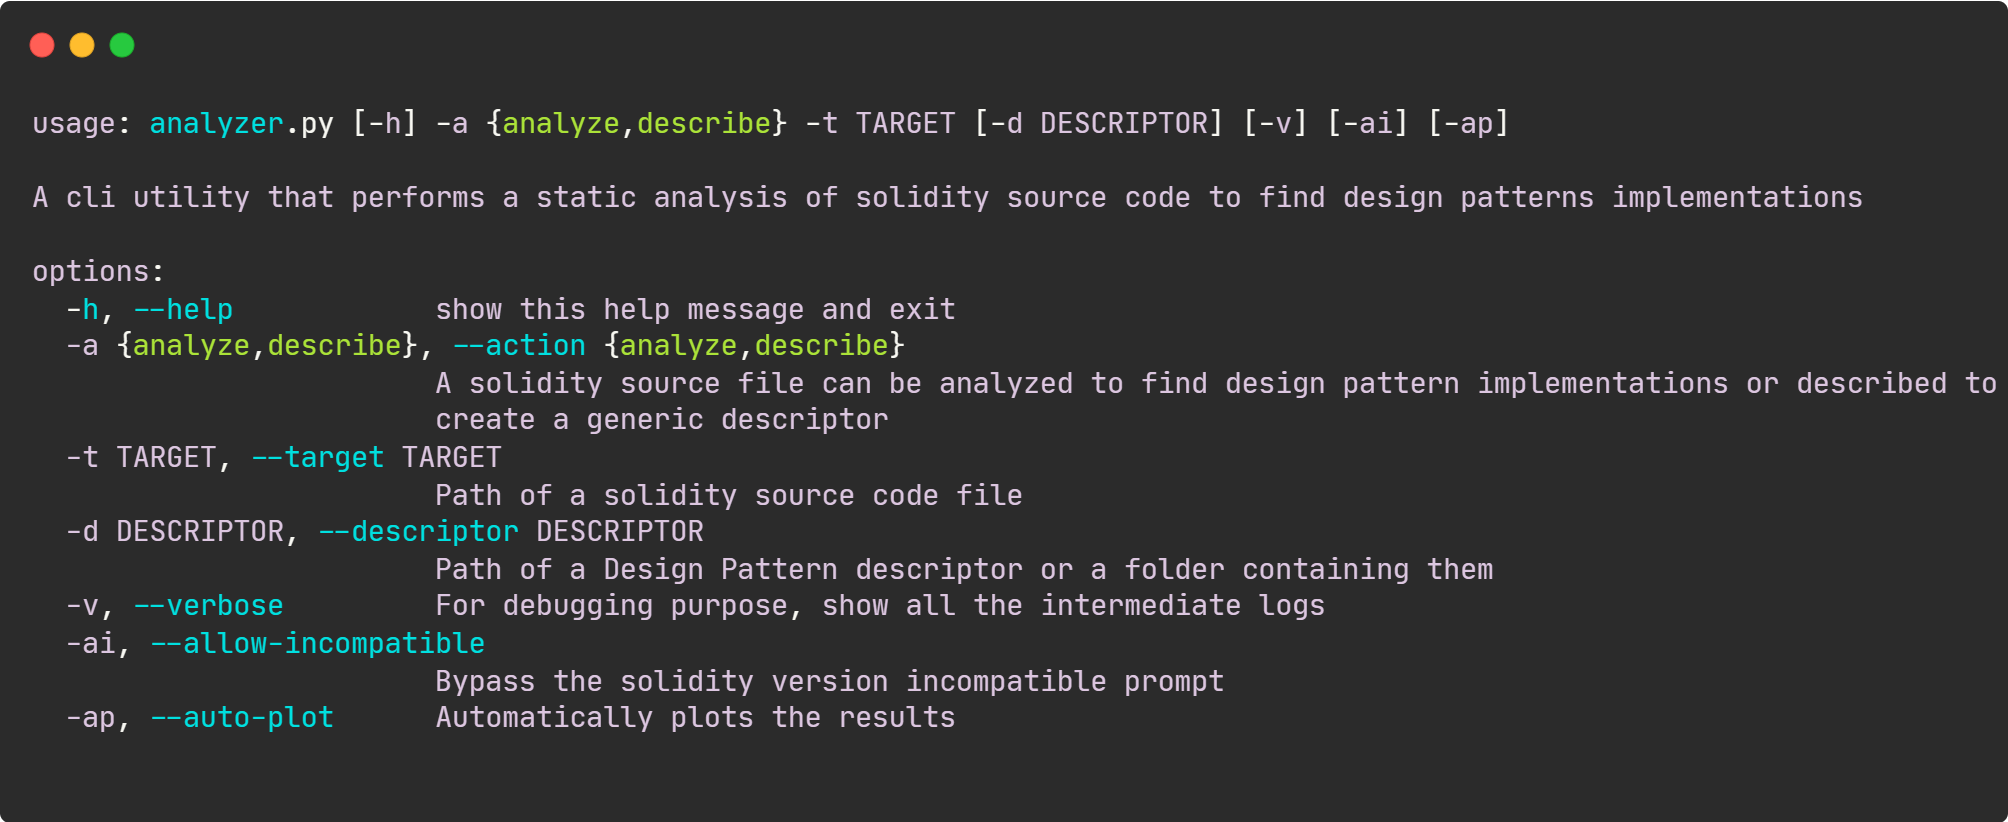
\includegraphics[width=\linewidth]{analyzer-tooltip}
	\caption{Manuale delle istruzioni di Analyzer}
	\label{analyzer-help-tip}
\end{figure}
L'applicativo software sviluppato è denominato \textit{"Solidity Design Pattern Analyzer"}, a cui, per semplicità, sarà fatto riferimento tramite l'abbreviazione \textit{"Analyzer"}.\\
\newline
Analyzer è un programma a riga di comando sviluppato in Python 3, e quindi supportato su MacOS, Linux e Windows, che prende in input il codice sorgente di un contratto, esegue una computazione e restituisce i risultati all'utente.\par
Lo scopo principale di Analyzer è automatizzare il processo di analisi statica del codice sorgente di uno smart-contract con l'obiettivo di individuare quali design pattern siano stati utilizzati.\par
Secondariamente, è possibile utilizzare Analyzer per \textit{descrivere} uno smart-contract, ovvero estrarre, tramite il processo di analisi statica, le informazioni utili a rappresentare un design pattern.

\section{Uso del programma}
Analyzer fa uso di librerie esterne, come ad esempio \textit{python-jsonschema}\cite{JSON-Schema} e \textit{matplotlib}. Per questo motivo, prima di poter utilizzare il programma è necessario installare tramite \textit{"pip"}, il package installer di Python, le dipendenze in uno dei seguenti modi:
\begin{itemize}
	\item \textit{Global Package}: installare le dipendenze direttamente nel sistema, diventando di fatto globali e accessibili da qualunque script Python eseguito nel sistema;
	\item \textit{Virtual Environment}: creare un ambiente virtuale in cui installare le dipendenze;
\end{itemize}
Una volta installate le dipendenze, per utilizzare Analyzer è necessario fornire una serie di parametri, qui elencati:
	\begin{table}[H]
	\centering
	\begin{tikzpicture}
		\node (table) [inner sep=0pt] {
			\def\arraystretch{1.5}
			\begin{tabular}{p{0.28\linewidth} | p{0.68\linewidth}}
				\textbf{-h, -\/-help} & {Un parametro \textit{opzionale} che, se fornito, farà stampare una guida sull'utilizzo nel terminale, così come mostrato in \mbox{Figura} \ref{analyzer-help-tip}.} \\ \hline
				\textbf{-a, -\/-action} & {Un parametro \textit{obbligatorio} che accetta soltanto i valori \textit\mbox{"analyze"} e \textit{"describe"}, a seconda dell'operazione che si vuole eseguire.} \\ \hline
				\textbf{-t, -\/-target} & {Un parametro \textit{obbligatorio} che rappresenta la \textit{path}, assoluta o relativa, del file contenente del codice sorgente Solidity.} \\ \hline
				\textbf{-d, -\/-descriptor} & {Un parametro \textit{obbligatorio} per l'operazione \textit{"analyze"} che rappresenta la \textit{path}, assoluta o relativa, del file o cartella contenente i \textit{"Design Pattern Descriptor"}. Se omesso verrà usato un \textit{path} predefinito.} \\ \hline
				\textbf{-v, -\/-verbose} & {Un parametro \textit{opzionale} che, se fornito, farà stampare nel terminale i log di debug, normalmente non visualizzati.} \\ \hline
				\textbf{-ai, \mbox{-\/-allow-incompatible}} & {Un parametro \textit{opzionale} che, se fornito, farà ignorare il controllo di compatibilità della versione di Solidity utilizzata nel file fornito.} \\ \hline
				\textbf{-ap, -\/-auto-plot} & {Un parametro \textit{opzionale} che, se fornito, farà visualizzare automaticamente il grafico dei risultati della ricerca dei design pattern.} \\
			\end{tabular}
		};
		\draw [rounded corners=.5em] (table.north west) rectangle (table.south east);
	\end{tikzpicture}
	\caption{Descrizione dei parametri di Analyzer}
\end{table}
\noindent Il parametro \textit{"action"} determina che tipo di operazione Analyzer debba eseguire sul file fornito:
\begin{itemize}
	\item \textit{analyze}: effettua la ricerca dell'utilizzo di design pattern e restituisce i risultati in formato JSON, opzionalmente è possibile visualizzare un grafico riassuntivo;
	\item \textit{describe}: estrae le informazioni utili a rappresentare un design pattern e restituisce i risultati in formato JSON, costituendo un \textit{descriptor};
\end{itemize}
Entrambe le operazioni si basano sulla tecnica di analisi statica.\par
Per esempio, volendo analizzare uno smart-contract al fine di individuare l'utilizzo dell'\textit{Ownership} pattern è necessario eseguire il comando:
\begin{lstlisting}[language=bash]
	$ python analyzer.py -a analyze -t ./source_code.sol -d ./Ownership_descriptor.json
\end{lstlisting}

\section{Applicazione dell'analisi statica}
Per eseguire l'analisi statica del codice sorgente fornito, Analyzer fa uso di una libreria esterna denominata \textit{"python-solidity-parser"}, che implementa un \textit{parser}, sperimentale e abbastanza acerbo, per il linguaggio di programmazione Solidity.\par
Tramite l'utilizzo del parser si effettua un controllo di correttezza sintattica del codice sorgente e si costruisce l'\textit{albero sintattico astratto} (\textit{AST}), una rappresentazione strutturata e gerarchica della sintassi del programma. Gli elementi del codice sono rappresentati come nodi dell'albero, dove ogni nodo rappresenta una porzione del codice e i suoi figli rappresentano porzioni più piccole e specifiche.
\newline

\noindent Con l'obiettivo di ottenere un sistema flessibile e facilmente estendibile, senza dover effettuare modifiche al codice sorgente di Analyzer, si è deciso di implementare, quando possibile, controlli generici.\par
L'utilizzo di controlli generici, con parametri configurabili, permette di definire un'unica logica applicabile alla ricerca di design pattern differenti.\par
Tale soluzione non è, però, sempre applicabile, infatti per specifici design pattern si è preferito implementare controlli specializzati al loro rilevamento.

\subsection{Controlli generici}
I controlli generici implementano la ricerca e disamina di elementi comuni, come ad esempio un confronto o l'utilizzo di modifier.\par
Viene esplorato l'albero sintattico astratto al fine di individuare i nodi di interesse, successivamente vengono estratte le informazioni utili e confrontate, mediante confronti \textit{case-insensitive} fra stringhe, con i parametri forniti.\par
Analyzer comprende i seguenti controlli generici: \textit{"comparison"}, \textit{"enum\textunderscore definition"}, \textit{"event\textunderscore emit"}, \textit{"fn\textunderscore call"}, \textit{"fn\textunderscore definition"}, \textit{"fn\textunderscore return\textunderscore parameters"}, \textit{"inheritance"}, \textit{"modifier"} e \textit{"state\textunderscore toggle"}.
\subsubsection{Comparison}
Questo controllo individua l'esecuzione di un'\textit{operazione di confronto} fra due operandi. Un'operazione di confronto fa uso di uno dei seguenti operatori: (==, !=, \textgreater, \textgreater =, \textless, \textless =).\par
Definita un'operazione di confronto, verrà automaticamente presa in considerazione anche quella con l'inversione dell'operatore equivalente.\par
Data la libertà implementativa, è possibile definire più di un'operazione di confronto, il controllo restituirà esito positivo al primo \textit{match} eseguito con successo.
Segue un esempio di parametrizzazione del controllo \textit{comparison}:
{\begin{lstlisting}[language=json, caption={Parametrizzazione del controllo Comparison}]
{
	"check_type": "comparison",
	"binary_operations": [
	{
		"operator": ">",
		"operand_1": "bilancio",
		"operand_2": "prelievo"
	}]
}\end{lstlisting}}
\noindent Tale controllo darà esito positivo per i confronti: \textit{bilancio\textgreater prelievo} e \textit{prelievo\textless bilancio}.\par
La verifica degli operandi viene effettuata assumendo che i parametri forniti debbano essere sotto-stringhe dei rispettivi operandi.

\subsubsection{Enum Definition}
Questo controllo individua la definizione di variabili di stato di tipo \textit{enum} denominati in modo specifico.\par
Possono essere forniti più nomi, il controllo restituirà esito positivo al primo \textit{match} eseguito con successo.
Segue un esempio di parametrizzazione:
{\begin{lstlisting}[language=json, caption={Parametrizzazione del controllo Enum Definition}]
{
	"check_type": "enum_definition",
	"enum_names": ["colori"]
}\end{lstlisting}}
\noindent Tale controllo darà esito positivo se all'interno del contratto è stato definito un \textit{enum} denominato \textit{"colori"}.\par
La verifica del nome dell'\textit{enum} viene effettuata assumendo che quest'ultimo sia contenuto nella lista dei parametri forniti. Si può definire un parametro come \textit{wildcard}, o sotto-stringa, concatenando il parametro stesso al simbolo '*': \textit{"colori*"}.


\subsubsection{Event emit}
Questo controllo individua l'emissione di di un evento.\par
Possono essere forniti molteplici nomi di eventi, il controllo restituirà esito positivo al primo \textit{match} eseguito con successo.
Segue un esempio di parametrizzazione:
{\begin{lstlisting}[language=json, caption={Parametrizzazione del controllo Event Emit}]
{
	"check_type": "event_emit",
	"enum_names": ["request*"]
}\end{lstlisting}}
\noindent Tale controllo darà esito positivo se all'interno del contratto viene emesso un evento il cui nome contiene la sotto-stringa \textit{"request"}.\par
Analogamente al controllo \textit{enum definition}, è possibile fornire come nome anche una stringa specifica.

\subsubsection{Function Call}
Questo controllo individua la chiamata di una funzione, con la possibilità di specificare o meno i suoi parametri.\par
Possono essere fornite svariate chiamate di funzione, il controllo restituirà esito positivo al primo \textit{match} eseguito con successo.
Segue un esempio di parametrizzazione:
{\begin{lstlisting}[language=json, caption={Parametrizzazione del controllo Function Call}]
{
	"check_type": "fn_call",
	"callable_function": ["require(*any*)"]
}\end{lstlisting}}
\noindent Tale controllo darà esito positivo se all'interno del contratto viene eseguita la funzione \textit{require} con qualunque tipo di parametro.\par
La stringa \textit{"*any*"} rappresenta una \textit{wildcard}, è possibile sostituirla con i parametri \textit{esatti} della funzione.

\subsubsection{Function Definition}
Questo controllo individua la definizione di una funzione denominata in modo specifico.\par
Possono essere forniti più nomi di funzione, il controllo restituirà esito positivo al primo \textit{match} eseguito con successo.
Segue un esempio di parametrizzazione:
{\begin{lstlisting}[language=json, caption={Parametrizzazione del controllo Function Definition}]
{
	"check_type": "fn_definition",
	"fn_names": ["commit", "reveal", "tracecommit"]
}\end{lstlisting}}
\noindent Tale controllo darà esito positivo se all'interno del contratto è stato definita una funzione il cui nome è presente nella lista nomi forniti.\par
Analogamente agli altri controlli, si può fornire come parametro una \textit{wildcard}, o sotto-stringa.

\subsubsection{Function Return Parameters}
Questo controllo individua la definizione di una funzione che ritorna una specifica serie di variabili.\par Possono essere forniti molteplici variabili di ritorno, specificando per ognuna il tipo e la collocazione nello storage, il controllo restituirà esito positivo solo se esiste una funziona che ritorni almeno tutte le variabili fornite come parametro.
Segue un esempio di parametrizzazione:
{\begin{lstlisting}[language=json, caption={Parametrizzazione del controllo Function Return Parameters}]
{
	"check_type": "fn_return_parameters",
	"parameters_list": [
	{
		"storage_location": "memory",
		"type": "ElementaryTypeName"
	}]
}\end{lstlisting}}
\noindent Tale controllo darà esito positivo se esiste una funzione che ritorna almeno un \textit{dato elementare} collocato in \textit{memory}.\par
Si può accettare qualunque collocazione dello storage ponendo come \textit{storage\textunderscore location} la \textit{wildcard} "*".

\subsubsection{Inheritance}
L'ereditarietà è un concetto importante della \textit{programmazione orientata agli oggetti} (\textit{OOP}). Consente di creare nuove classi a partire da classi esistenti, ereditandone le proprietà e i comportamenti. Questo rende più semplice la creazione di nuove classi e la manutenzione del codice, poiché è possibile riutilizzare e modificare il codice esistente invece di creare tutto da zero.\par
Solidity supporta l'ereditarietà tra smart-contract, dove più contratti possono essere ereditati in un singolo contratto. Il contratto da cui gli altri contratti ereditano le caratteristiche è noto come \textit{contratto base}, mentre il contratto che eredita le caratteristiche è detto \textit{contratto derivato}:
\begin{itemize}
	\item Un \textit{contratto derivato} può accedere a tutti i membri non privati, comprese le variabili di stato, i funzioni interni e modifier;
	\item L'\textit{overriding} delle funzioni è consentitp a condizione che la firma della funzione rimanga la stessa;
	\item Si può chiamare la funzione di un contratto base usando la parola chiave \textit{super} o il nome del \textit{contratto base}.
\end{itemize}
Questo controllo individua la singola o multipla ereditarietà del contratto fornito e confronta il nome dei \textit{contratti base} ottenuti con una lista di nomi fornita come parametro.\par
Costituisce uno dei controlli più utilizzati in combinazione con gli altri, in quanto, supponendo l'utilizzo di libreria come \textit{OpenZeppelin}\cite{openzeppelin}, è più probabile ereditare le caratteristiche di un design pattern anziché implementarle da zero.\par
Possono essere forniti più nomi di \textit{contratti base}, il controllo restituirà esito positivo al primo \textit{match} eseguito con successo.
Segue un esempio di parametrizzazione:
{\begin{lstlisting}[language=json, caption={Parametrizzazione del controllo Inheritance}]
{
	"check_type": "inheritance",
	"parent_names": ["deprecatable"]
}\end{lstlisting}}
\noindent Tale controllo darà esito positivo se il contratto che si sta analizzando eredità le proprietà e le caratteristiche di un contratto denominato \textit{"Deprecatable"}.\par
Analogamente agli altri controlli, è possibile fornire come nome anche una \textit{wildcard}.

\subsubsection{Modifier}
Questo controllo individua la definizione o l'utilizzo di modifier denominati in modo specifico.\par
Possono essere forniti più nomi di \textit{modifier}, il controllo restituirà esito positivo al primo \textit{match} eseguito con successo.
Segue un esempio di parametrizzazione:
{\begin{lstlisting}[language=json, caption={Parametrizzazione del controllo Modifier}]
{
	"check_type": "modifier",
	"modifiers": ["when*", "after*"]
}\end{lstlisting}}
\noindent Tale controllo darà esito positivo se esiste almeno una funzione che utilizza almeno uno dei modifier forniti come parametro.\par
Analogamente agli altri controlli, è possibile fornire anche un nome specifico.

\subsubsection{State Toggle}
Questo controllo individua l'utilizzo di un interruttore software. L'interruttore è rappresentato da una variabile di stato \textit{booleana} e da una funzione che ne esegue il \textit{flip}.\par
Data la libertà implementativa, viene riconosciuto il \textit{flip} più comunemente utilizzato, basato sull'operatore di negazione (\textit{state\textunderscore bool = !state\textunderscore bool}).\par
Possono essere forniti più nomi di variabile, il controllo restituirà esito positivo al primo \textit{match} eseguito con successo.
Segue un esempio di parametrizzazione:
{\begin{lstlisting}[language=json, caption={Parametrizzazione del controllo Comparison}]
{
	"check_type": "state_toggle",
	"state_names": ["paused*"]
}\end{lstlisting}}
\noindent Tale controllo darà esito positivo se esistono una variabile di stato booleana che nel nome contiene \textit{"paused"} e un'istruzione di \textit{flip} relativa.\par
Analogamente agli altri controlli, è possibile fornire anche un nome specifico.

\subsection{Controlli specializzati}
I controlli specializzati implementano la ricerca e disamina di elementi specifici, difficilmente rappresentabili come elementi semplici, come ad esempio la distanza fra una funzione esterna e un assegnamento o il packing delle variabili.\par
Analyzer comprende i seguenti controlli specializzati: \textit{"check\textunderscore effects\textunderscore interaction"}, \textit{"eternal\textunderscore storage"}, \textit{"memory\textunderscore array\textunderscore building"}, \textit{"rejector"}, \textit{"relay"} e \textit{"tight\textunderscore variable\textunderscore packing"}
\subsubsection{Check Effects Interaction}
Questo controllo individua l'omonimo design pattern.\par Ricerca una chiamata alle funzioni esterne offerte da Solidity, ovvero l'utilizzo delle funzioni \textit{call()}, \textit{send()} e \textit{transfer()}, preceduta da un'istruzione di assegnamento.\par Al fine di affinare la probabilità di rilevamento e diminuire i casi falsi positivi, si è definita una distanza massima di cinque righe.
{\begin{lstlisting}[language=json, caption={Controllo Check Effects Interaction}]
{ "check_type": "check_effects_interaction" }\end{lstlisting}}

\subsubsection{Eternal Storage}
Questo controllo individua il \textit{Data Segregation} pattern, conosciuto anche come \textit{Eternal Storage}.\par Data la libertà implementativa, il controllo è incentrato sulla ricerca di \textit{mapping} e la definizione delle funzioni di supporto \textit{getter} e \textit{setter}.\par
Il nome delle funzioni di supporto è definito come il nome del mapping preceduto rispettivamente da \textit{"get"} e \textit{"set"}.\par
Nell'EVM, un mapping definito con visibilità \textit{pubblica} genera automaticamente un \textit{getter}, viene, perciò, gestito anche il caso in cui non vi sia l'esplicita definizione del \textit{getter}. 
{\begin{lstlisting}[language=json, caption={Controllo Eternal Storage}]
{ "check_type": "eternal_storage" }\end{lstlisting}}
	
\subsubsection{Memory Array Building}
Questo controllo individua l'omonimo design pattern.\par Ricerca la definizione di una funzione con modifier \textit{view} che ritorni un array collocato in \textit{memory}.
{\begin{lstlisting}[language=json, caption={Controllo Memory Array Building}]
{ "check_type": "memory_array_building" }\end{lstlisting}}
	
\subsubsection{Rejector}
Questo controllo individua l'omonimo design pattern.\par Verifica che il contratto fornito implementi \textit{solo} la funzione di \textit{fallback()} in cui viene eseguita la funzione \textit{revert()}.
{\begin{lstlisting}[language=json, caption={Controllo Rejector}]
{ "check_type": "rejector" }\end{lstlisting}}
	
\subsubsection{Relay}
Questo controllo individua sia il \textit{Relay} pattern sia il \textit{Register} pattern.\par Verifica che il contratto fornito implementi la funzione di \textit{fallback()} in cui viene eseguita la funzione \textit{delegatecall()}.
{\begin{lstlisting}[language=json, caption={Controllo Relay}]
{ "check_type": "relay" }\end{lstlisting}}
	
\subsubsection{Tight Variable Packing}
Questo controllo individua l'omonimo design pattern.\par Ricerca la definizione di una \textit{struct} contenente tipi di dati la cui somma delle dimensioni sia minore o uguale, quando possibile, a 32 byte.\par
Le \textit{struct} contenenti almeno un elemento di dimensione dinamica, come ad esempio array o numeri a virgola mobile, vengono scartate, in quanto non è possibile valutarne la dimensione a priori.
{\begin{lstlisting}[language=json, caption={Controllo Tight Variable Packing}]
{ "check_type": "tight_variable_packing" }\end{lstlisting}}

\section{Design Pattern Descriptor}
Stabiliti i controlli supportati da Analyzer, è possibile definire un \textit{Design Pattern Descriptor} come un \textit{oggetto JSON} contenente una raccolta di uno o più controlli opportunatamente parametrizzati al fine di individuare uno specifico design pattern.\par
Come esempio, si riporta il descriptor dell'\textit{Auto Deprecation} pattern:
	{\begin{lstlisting}[language=json, caption={Auto Deprecation Descriptor}, label={descriptor:auto_deprecation}]
{
	"name": "Auto Deprecation",
	"checks": [
	{
		"check_type": "inheritance",
		"parent_names": ["deprecatable"]
	},
	{
		"check_type": "modifier",
		"modifiers": ["willDeprecate", "whenDeprecated"]
	},
	{
		"check_type": "comparison",
		"binary_operations": [
		{
			"operator": ">",
			"operand_1": "timestamp",
			"operand_2": "expire"
		}]
	}]
}\end{lstlisting}}
\subsection{Affinamento dei parametri}
Per individuare un design pattern, la correttezza dei parametri dei controlli utilizzati è fondamentale. Un parametro troppo generico può causare dei falsi positivi, viceversa può ridurre le probabilità di riconoscimento.\par
Al fine di migliorare i parametri, estratti dai codici di riferimento riportati in \hyperref[appendix:codici]{Appendice}, si è analizzata la libreria \textit{OpenZeppelin Contracts}\cite{openzeppelin}, una libreria per lo sviluppo di smart-contract sicuri, costituita da una solida codebase verificata dalla comunità.\par Data la sua diffusione, si è utilizzato Analyzer per estrarre informazioni utili da utilizzare come ulteriori parametri.

\subsection{Validazione tramite JSONSchema}
Un descriptor descrive le caratteristiche principali di un design pattern e permette ad Analyzer di rilevarne l'utilizzo.\par 
Inoltre, allo scopo di rilevare nuovi design pattern, non riconosciuti da Analyzer, l'utente può definire, basandosi sui controlli supportati, nuovi descriptor.\\
\newline
Data la natura configurabile dei descriptor, nasce il rischio di incorrere in descriptor malformati o contenenti dati incoerenti, di conseguenza vi è la necessità di validarli in maniera semplice ed efficace.\par Per la convalida, Analyzer utilizza la libreria esterna denominata \textit{"python-jsonschema"} \cite{python-jsonschema} e lo schema \ref{appendix:json_schema}, riportato in \hyperref[appendix:codici]{Appendice}:
\begin{lstlisting}[language=Python, caption={Istruzione di validazione}]
jsonschema.validate(instance=descriptor_object, schema=self._descriptor_schema)
\end{lstlisting}
\noindent A scopo informativo, si riporta e commenta la porzione di schema che modella i dati del controllo \textit{"comparison"}, di cui vi è un utilizzo nel codice \ref{descriptor:auto_deprecation}:
{\begin{lstlisting}[language=json, caption={JSONSchema del controllo "comparison"}]
{
	"type": "object",
	"properties": { 
		"check_type": { "type": "string", "const": "comparison" },
		"binary_operations": {
			"type": "array",
			"items": [
			{
				"type": "object",
				"properties": { 
					"operator": { "type": "string" },
					"operand_1": { "type": "string" },
					"operand_2": { "type": "string" }
				},
				"required": [ "operator", "operand_1", "operand_2" ]
			}],
			"uniqueItems": true, "minItems": 1
		}
	},
	"required": [ "check_type", "binary_operations" ]},\end{lstlisting}}  
\noindent Questo modello descrive un oggetto JSON che deve soddisfare le seguenti regole:
\begin{itemize}
		\item {L'oggetto deve contenere le proprietà \textit{"check\textunderscore type"} e \textit{"binary\textunderscore operations"}, rispettivamente una \textit{stringa} di valore \textit{"comparison"} e un \textit{array JSON} di oggetti JSON, rappresentanti le operazioni binarie. Entrambe le proprietà sono obbligatorie;} 
		\item Un'operazione binaria è rappresentata da un oggetto JSON contenente le proprietà di tipo stringa \textit{"operator"}, \textit{"operand\textunderscore 1"} e \textit{operand\textunderscore 2}, tutte e tre obbligatorie;
		\item L'array JSON di operazioni binarie deve contenere almeno un elemento e tutti gli elementi devono essere distinti;
\end{itemize}
\section{Ricerca di Design Pattern}
Fornendo il valore \textit{"analyze"} come parametro \textit{"action"} viene effettuata la ricerca di design pattern nel codice sorgente fornito in input. L'esecuzione di questa operazione può essere essenzialmente suddivisa in tre fasi:
\begin{itemize}
	\item \textit{Bootstrap}: in questa fase vengono convalidati i parametri forniti dall'utente;
	\item \textit{Parsing e Analisi}: in questa fase vengono eseguiti il parsing del codice sorgente e la ricerca dei design pattern;
	\item \textit{Report dei risultati}: in questa fase vengono mostrati all'utente i risultati della ricerca, opzionalmente può essere mostrato un grafico riassuntivo;
\end{itemize}

\subsection{Fase di Bootstrap}
Nella fase di \textit{bootstrap} vengono verificati i parametri forniti dall'utente.\par
Viene verificata l'estensione dei file, affinché il parametro \textit{target} sia un file sorgente Solidity, e il parametro \textit{descriptor} sia un file \textit{json} o una cartella, contenente file \textit{json}.\par
Successivamente, i descriptor forniti vengono validati mediante lo schema \ref{appendix:json_schema}, riportato in \hyperref[appendix:codici]{Appendice}. I descriptor non validati vengono ignorati e non utilizzati nella fase successiva.\par
In caso di parametri invalidi, od omessi, viene restituito un messaggio d'errore esplicativo e, in caso di errore critico, viene terminato il processo.
\newpage
\subsection{Fase di Parsing e Analisi}
Nella fase di \textit{parsing e analisi}, mediante l'utilizzo del parser, viene effettuato un controllo di correttezza della sintassi e costruito l'albero sintattico astratto.\par
Successivamente, vengono eseguiti i controlli contenuti in ogni descriptor precedentemente convalidato, tenendo traccia di quali controlli hanno avuto esito positivo.\par
In caso di errori di sintassi all'interno del codice sorgente il processo viene terminato.

\subsection{Fase di Report dei risultati}
Nella fase di \textit{report dei risultati}, viene stampato sul terminale una sintesi dell'esito dei controlli eseguiti. Inoltre, tale sintesi viene salvata sul disco in formato JSON, nello stesso \textit{path} del file sorgente fornito in input.\par
L'esito positivo di uno dei controllo di un descriptor suggerisce, in quanto non è possibile fornire la certezza, che il design pattern rappresentato potrebbe essere in uso.\par
Opzionalmente, è possibile visualizzare la sintesi sotto forma di grafico.
\newline
Segue un esempio di sintesi in formato JSON:
{\begin{lstlisting}[language=json, caption={Report del codice di riferimento dell'Ownership}, label={report:ownership-text}]
{"Ownable":{
	"AccessRestriction":{"inheritance":false,"modifier":true},
	"AutoDeprecation":{"inheritance":false,"modifier":false,"comparison":false},
	"BalanceLimit":{"comparison":false},
	"CheckEffectsInteraction":{"check_effects_interaction":false},
	"CircuitBreaker":{
		"inheritance":false,
		"state_toggle":false,
		"fn_definition":false,
		"modifier":false
	},
	"CommitReveal":{
		"fn_call":false,
		"fn_definition":false,
		"event_emit":false
	},
	"EternalStorage":{"eternal_storage":false},
	"GuardCheck":{"fn_call":true},
	"MemoryArrayBuilding":{"memory_array_building":false},
	"Mortal":{"inheritance":false,"fn_call":false},
	"Mutex":{"inheritance":false,"modifier":false,"fn_definition":false},
	"Oracle":{"fn_call":false,"fn_definition":false,"event_emit":false},
	"Ownership":{"inheritance":false,"modifier":true,"comparison":true},
	"PullOverPush":{"inheritance":false,"fn_call":false},
	"Randomness":{"fn_call":false},
	"RateLimit":{"modifier":false,"inheritance":false},
	"Rejector":{"rejector":false},
	"Relay":{"inheritance":false,"relay":false},
	"SecureTransfer":{"fn_call":false},
	"StateMachine":{"modifier":false,"enum_definition":false,"fn_definition":false},
	"StringEquality":{"comparison":false},
	"TightVariablePacking":{"tight_variable_packing":false}
}}\end{lstlisting}
Il report testuale mostrato nel Codice \ref{report:ownership-text} può essere visualizzato in forma di grafico a barre:
\begin{figure}[H]
	\centering
	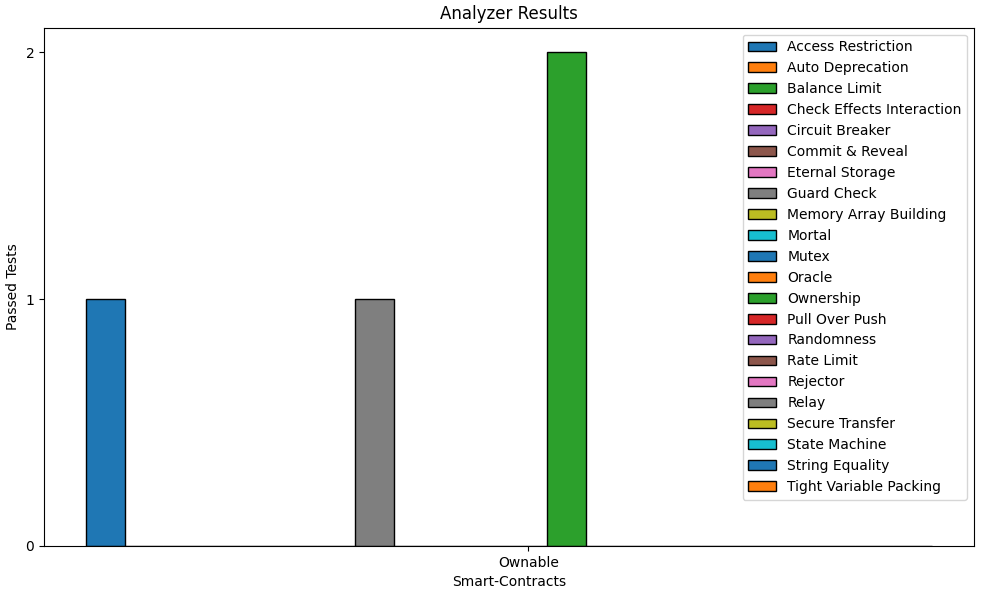
\includegraphics[width=\linewidth]{ownership-plot}
	\caption{Grafico a barre dell'analisi del codice di riferimento dell'Ownership}
\end{figure}

\section{Descrizione di uno smart-contract}
Fornendo il valore \textit{"describe"} come parametro \textit{"action"} viene effettuata descrizione dello smart-contract. \par
La descrizione consiste nel generare un descriptor con le informazioni utili estratte mediante l'analisi statica. Analogamente alla ricerca dei design pattern, l'esecuzione di questa operazione può essere similmente suddivisa in tre fasi:
\begin{itemize}
	\item \textit{Bootstrap}: in questa fase vengono convalidati i parametri forniti dall'utente;
	\item \textit{Parsing e Analisi}: in questa fase vengono eseguiti il parsing del codice sorgente e l'estrazione delle informazioni utili;
	\item \textit{Generazione del descriptor}: in questa fase generato e salvato il descriptor costituito dalle informazioni estratte;
\end{itemize}

\subsection{Fase di Bootstrap}
Analoga alla fase di \textit{bootstrap} della ricerca di design pattern.\par
Dato che l'operazione \textit{"describe"} non richiede alcun descriptor come input, viene verificata soltanto l'estensione del file sorgente Solidity.

\subsection{Fase di Parsing e Analisi}
Analogamente alla fase di \textit{parsing e analisi} della ricerca di design pattern, viene effettuato un controllo di correttezza della sintassi e costruito l'albero sintattico astratto.\par
Successivamente, viene eseguita una serie di funzioni di supporto per estrarre tutti i possibili parametri dei \textit{controlli generici}.\par
In caso di errori di sintassi all'interno del codice sorgente il processo viene terminato.

\subsection{Fase di Generazione del descriptor}
Nella fase di \textit{generazione del descriptor}, le informazioni utili estratte vengono raccolte in un descriptor, il quale viene salvato sul disco nello stesso \textit{path} del file sorgente fornito in input.\par
Segue il descriptor generato usando il codice \ref{appendix:ownership}:
{\begin{lstlisting}[language=json, caption={Report del codice di riferimento dell'Ownership}]
{
	"name": "Ownable",
	"checks": [
	{
		"check_type": "comparison",
		"binary_operations": [
		{
			"operator": "==",
			"operand_1": "_owner",
			"operand_2": "msg.sender"
		}
		]
	},
	{ "check_type": "modifier", "modifiers": [ "onlyowner" ] },
	{
		"check_type": "fn_call",
		"callable_function": [
			"address(0)",
			"require(_owner == msg.sender, \"ownable: caller is not the owner\")",
			"ownershiptransferred(address(0), _owner)"
		]
	},
	{ "check_type": "fn_definition", "fn_names": [ "constructor" ] },
	{ "check_type": "event_emit", "event_names": [ "ownershiptransferred" ] }]
}\end{lstlisting}



\begin{frontmatter}
\pagenumbering{arabic} \setcounter{page}{42}
\chapter{Conclusioni}
Termina così lo sviluppo dell'applicativo software proposto nella tesi.\\
\newline
\textit{Solidity Design Pattern Analyzer} è un software \textit{open-source} rilasciato con licenza \textit{MIT}, il cui codice sorgente è liberalmente accessibile nel relativo repository su GitHub\cite{github-repo}.\\
\newline
L'applicativo software è in grado di eseguire le seguenti operazioni:
\begin{itemize}
	\item Rilevare, nei limiti linguistici e delle dipendenze utilizzate, tutti e ventidue i design pattern documentati nella tesi, i cui relativi descriptor sono inclusi nel codice sorgente, ed è possibile, mediante la combinazione di controlli generici, definire nuovi descriptor per riconoscere design pattern futuri;
	\item Descrivere uno smart-contract, ovvero estrarre le informazioni utili a creare un nuovo descriptor;
\end{itemize} 
Si conclude la tesi elencando un'ipotetica serie di sviluppi futuri:
\begin{itemize}
	\item Introdurre il supporto di dizionari di lingue diverse dall'inglese al fine di permettere l'analisi degli smart-contract le cui informazioni utili, come nomi di variabili di stato o di funzioni, corrispondono a parole di lingue straniere;
	\item Implementare un sistema di raggruppamento e interdipendenza dei controlli allo scopo di rilevare costrutti più articolati;
	\item Progettare un'interfaccia grafica per un utilizzo più user-friendly dell'applicativo;
\end{itemize}
 
 
\printbibliography[heading=bibintoc]
\appendix
\chapter{Appendice}
\setcounter{secnumdepth}{0}
{\section{Codice di riferimento degli Authorization Design Pattern}\label{appendix:codici}

{\label{appendix:access_restriction}
	\begin{lstlisting}[language=Solidity, caption={Codice di riferimento per Access Restriction}]
contract AccessRestriction {
	uint256 public creationTime = block.timestamp;
	modifier onlyBefore(uint256 _time) {
		require(block.timestamp < _time);
		_;
	}
	modifier minAmount(uint256 _amount) {
		require(msg.value >= _amount);
		_;
	}
	function test() public payable onlyBefore(creationTime + 10 seconds) minAmount(1 ether) {
		// Do something
	}
}
\end{lstlisting}}

{\label{appendix:ownership}\begin{lstlisting}[language=Solidity, caption={Codice di riferimento per Ownership}]
contract Ownable {
	address private _owner;
	event OwnershipTransferred(address indexed previousOwner, address indexed newOwner);
	constructor() {
		_owner = msg.sender;
		emit OwnershipTransferred(address(0), _owner);
	}
	modifier onlyOwner() {
		require(_owner == msg.sender, "Ownable: caller is not the owner");
		_;
	}
}
\end{lstlisting}}
}
\newpage
{\section{Codice di riferimento dei Behavioral Design Pattern}

{\label{appendix:commit_and_reveal}\begin{lstlisting}[language=Solidity, caption={Codice di riferimento per Commit and Reveal}]
contract CommitReveal {
	struct Commit {string choice; string secret; string status;}
	mapping(address => mapping(bytes32 => Commit)) public userCommits;
	event LogCommit(bytes32, address);
	event LogReveal(bytes32, address, string, string);
	function commit(bytes32 _commit) public returns (bool success) {
		Commit storage userCommit = userCommits[msg.sender][_commit];
		if (bytes(userCommit.status).length != 0)
			return false;
		userCommit.status = "c";
		emit LogCommit(_commit, msg.sender);
		return true;
	}
	function reveal(string calldata _choice, string calldata _secret, bytes32 _commit) public returns (bool success) {
		Commit storage userCommit = userCommits[msg.sender][_commit];
		bytes memory bytesStatus = bytes(userCommit.status);
		if (bytesStatus.length == 0)
			return false;
		else if (bytesStatus[0] == "r")
			return false;
		if (_commit != keccak256(abi.encodePacked(_choice, _secret)))
			return false; 
		userCommit.choice = _choice;
		userCommit.secret = _secret;
		userCommit.status = "r";
		emit LogReveal(_commit, msg.sender, _choice, _secret);
		return true;
	}
	function traceCommit(address _address, bytes32 _commit) public view
	returns (string memory choice, string memory secret, string memory status) {
		Commit storage userCommit = userCommits[_address][_commit];
		require(bytes(userCommit.status)[0] == "r");
		return (userCommit.choice, userCommit.secret, userCommit.status);
	}
}
\end{lstlisting}}

{\label{appendix:guardcheck}\begin{lstlisting}[language=Solidity, caption={Codice di riferimento per GuardCheck}]
contract GuardCheck {
	function donate(address addr) payable public {
		require(addr != address(0));
		require(msg.value != 0);
		uint balanceBeforeTransfer = address(this).balance;
		uint transferAmount;
		if (addr.balance == 0) {
			transferAmount = msg.value;
		} else if (addr.balance < msg.sender.balance) {
			transferAmount = msg.value / 2;
		} else {
			revert();
		}
		payable(addr).transfer(transferAmount);
		assert(address(this).balance == balanceBeforeTransfer - transferAmount);      
	}
}
\end{lstlisting}}

{\label{appendix:oracle}\begin{lstlisting}[language=Solidity, caption={Codice di riferimento per Oracle}]
contract Oracle {
	address knownSource = address(0x1234);
	struct Request {
		bytes data;
		function(bytes memory) external callback;
	}
	Request[] requests;
	event NewRequest(uint256);
	modifier onlyBy(address account) {
		require(msg.sender == account);
		_;
	}
	function query(bytes memory data, function(bytes memory) external callback) public
	{
		requests.push(Request(data, callback));
		emit NewRequest(requests.length - 1);
	}
	function reply(uint256 requestID, bytes memory response) public onlyBy(knownSource)
	{
		requests[requestID].callback(response);
	}
}
contract OracleConsumer {
	Oracle oracle = Oracle(address(0x4321));
	modifier onlyBy(address account) { 
		require(msg.sender == account);  _; 
	}
	function updateExchangeRate() public {
		oracle.query("USD", this.oracleResponse);
	}
	function oracleResponse(bytes memory response) public onlyBy(address(oracle)) {
		// do something with response
	}
}
\end{lstlisting}}

{\label{appendix:pull_over_push}\begin{lstlisting}[language=Solidity, caption={Codice di riferimento per Pull Over Push}]
contract Auction {
	address public highestBidder;
	uint highestBid;
	mapping(address => uint) refunds;
	function bid() public payable {
		require(msg.value >= highestBid);
		if (highestBidder != address(0)) {
			refunds[highestBidder] += highestBid; 
		}
		highestBidder = msg.sender;
		highestBid = msg.value;
	}
	function withdrawRefund() public {
		uint refund = refunds[msg.sender];
		refunds[msg.sender] = 0;
		payable(msg.sender).transfer(refund);
	}
}
\end{lstlisting}}

\newpage

{\label{appendix:randomness}\begin{lstlisting}[language=Solidity, caption={Codice di riferimento per Randomness}]
contract SimpleRandom {
	function simpleRandomNumber() internal view returns (uint) {
		return uint(blockhash(block.number - 1));
	}
	function seededRandomNumber(string calldata seed) internal view returns (uint) {
		return uint(keccak256(abi.encodePacked(blockhash(block.number-1), seed)));
	}
	function random() public view returns (uint) {
		return uint(keccak256(abi.encodePacked(block.timestamp, msg.sender, block.difficulty)));
	}
}
\end{lstlisting}}

{\label{appendix:state_machine}\begin{lstlisting}[language=Solidity, caption={Codice di riferimento per State Machine}]
contract DepositLock {
	enum Stages {
		AcceptingDeposits,
		FreezingDeposits,
		ReleasingDeposits
	}
	Stages public stage = Stages.AcceptingDeposits;
	uint256 public creationTime = block.timestamp;
	mapping(address => uint256) balances;
	
	modifier atStage(Stages _stage) {
		require(stage == _stage);
		_;
	}
	modifier timedTransitions() {
		if (stage == Stages.AcceptingDeposits && block.timestamp >= creationTime + 1 days) nextStage();
		if (stage == Stages.FreezingDeposits && block.timestamp >= creationTime + 8 days) nextStage();
		_;
	}
	function nextStage() internal {
		stage = Stages(uint256(stage) + 1);
	}
	function deposit() public payable timedTransitions atStage(Stages.AcceptingDeposits) {
		balances[msg.sender] += msg.value;
	}
	
	function withdraw() public timedTransitions atStage(Stages.ReleasingDeposits) {
		uint256 amount = balances[msg.sender];
		balances[msg.sender] = 0;
		payable(msg.sender).transfer(amount);
	}
}
\end{lstlisting}}}
\newpage
{\section{Codice di riferimento dei Gas Economic Design Pattern}

{\label{appendix:memory_array_building}\begin{lstlisting}[language=Solidity, caption={Codice di riferimento per Memory Array Building}]
contract MemoryArrayBuilding {
	struct Item {
		string name;
		string category;
		address owner;
		uint32 zipcode;
		uint32 price;
	}
	Item[] public items;
	mapping(address => uint) public ownerItemCount;
	function getItemIDsByOwner(address _owner) public view returns (uint[] memory) {
		uint[] memory result = new uint[](ownerItemCount[_owner]);
		uint counter = 0;
		for (uint i = 0; i < items.length; i++) {
			if (items[i].owner == _owner) {
				result[counter] = i;
				counter++;
			}
		}
		return result;
	}
}
\end{lstlisting}}

{\label{appendix:string_equality_comparison}\begin{lstlisting}[language=Solidity, caption={Codice di riferimento per String Equality Comparison}]
contract SimpleContractExample {
	function hashCompareCheck(string memory _a, string memory _b) internal pure returns (bool) {
		return
		keccak256(abi.encodePacked(_a)) == keccak256(abi.encodePacked(_b));
	}
	function hashCompareWithLengthCheck(string memory _a, string memory _b) internal pure returns (bool) {
		if (bytes(_a).length != bytes(_b).length) {
			return false;
		} else {
			return keccak256(abi.encodePacked(_a)) == keccak256(abi.encodePacked(_b));
		}
	}
}
\end{lstlisting}}
\newpage
{\label{appendix:tight_variable_packing}\begin{lstlisting}[language=Solidity, caption={Codice di riferimento per Tight Variable Packing}]
contract StructPackingExample {
	struct CheapStruct {
		uint8 a;
		uint8 b;
		uint8 c;
		uint8 d;
		bytes1 e;
		bytes1 f;
		bytes1 g;
		bytes1 h;
	}
	CheapStruct example;
	function addCheapStruct() public {
		CheapStruct memory someStruct = CheapStruct(1,2,3,4,"a","b","c","d");
		example = someStruct;
	}
}
\end{lstlisting}}}
{\section{Codice di riferimento dei Lifecycle Design Pattern}

{\label{appendix:auto_deprecation}\begin{lstlisting}[language=Solidity, caption={Codice di riferimento per Auto Deprecation}]
contract Deprecatable {
	uint expires;
	constructor(uint _lifetime) { 
		expires = block.timestamp + _lifetime;
	}
	function expired() public view returns (bool) { 
		return block.timestamp > expires ? true : false;
	}
	modifier willDeprecate() { 
		if (!expired()) {_;}
	}
	modifier whenDeprecated() { 
		if (expired()) {_;}
	}
}
\end{lstlisting}}

{\label{appendix:mortal}\begin{lstlisting}[language=Solidity, caption={Codice di riferimento per Mortal}]
contract Mortal is Ownable {
	function destroy() public onlyOwner { 
		selfdestruct(payable(_owner)); 
	}
	function destroyWithoutModifier() public {
		if (msg.sender == owner())
		selfdestruct(payable(_owner)); 
	}
}
\end{lstlisting}}}
\newpage
{\section{Codice di riferimento dei Maintenance Design Pattern}

{\label{appendix:data_segregation}\begin{lstlisting}[language=Solidity, caption={Codice di riferimento per Data Segregation}]
contract Storage {
	mapping(bytes32 => uint256) public uintStorage;
	mapping(bytes32 => address) public addressStorage;
	function setUintStorage(bytes32 key, uint256 value) public {
		uintStorage[key] = value;
	}
	function setaddressStorage(bytes32 key, address value) public {
		addressStorage[key] = value;
	}
}
contract Logic {
	Storage _storage;
	constructor(address storageAddress) {
		_storage = Storage(storageAddress);
	}
	function test() public returns (uint256) {
		bytes32 key = keccak256("capybara");
		_storage.setUintStorage(key, 911);
		return _storage.uintStorage(key);
	}
}
\end{lstlisting}}

{\label{appendix:register}\begin{lstlisting}[language=Solidity, caption={Codice di riferimento per Register}]
contract Register is Ownable {
	address public currentVersion;
	address[] previousVersions;
	function updateContract(address newVersion) public onlyOwner returns (bool) {
		if (newVersion != currentVersion) {
			previousVersions.push(currentVersion);
			currentVersion = newVersion;
			return true;
		}
		return false;
	}
	fallback() external {
		(bool success, ) = currentVersion.delegatecall(msg.data);
		require(success);
	}
}
\end{lstlisting}}

{\label{appendix:relay}\begin{lstlisting}[language=Solidity, caption={Codice di riferimento per Relay}]
contract Relay is Ownable {
	address public currentVersion;
	constructor(address initAddr) { currentVersion = initAddr; }
	function updateContract(address newVersion) public onlyOwner {
		currentVersion = newVersion;
	}
	fallback() external {
		(bool success, ) = currentVersion.delegatecall(msg.data);
		require(success);
	}
}
\end{lstlisting}}
}
{\section{Codice di riferimento dei Security Design Pattern}

{\label{appendix:balance_limit}\begin{lstlisting}[language=Solidity, caption={Codice di riferimento per Balance Limit}]
contract BalanceLimit {
	uint256 limit;
	constructor(uint256 _value) {
		limit = _value;
	}
	modifier limitedPayable() {
		require(address(this).balance <= limit);
		_;
	}
	function deposit() public payable limitedPayable {
		// TO-DO Something
	}
}
\end{lstlisting}}

{\label{appendix:check_effects_interactions}\begin{lstlisting}[language=Solidity, caption={Codice di riferimento per Check Effects Interactions}]
contract ChecksEffectsInteractions {
	mapping(address => uint256) balances;
	function deposit() public payable {
		balances[msg.sender] = msg.value;
	}
	function withdraw(uint256 amount) public {
		require(balances[msg.sender] >= amount);
		balances[msg.sender] -= amount;
		payable(msg.sender).transfer(amount);
	}
}
\end{lstlisting}}

\label{appendix:emergency_stop}{\begin{lstlisting}[language=Solidity, caption={Codice di riferimento per Emergency Stop}]
contract EmergencyStop is Ownable {
	bool private contractStopped = false;
	modifier haltInEmergency() {
		if (!contractStopped) _;
	}
	modifier enableInEmergency() {
		if (contractStopped) _;
	}
	function toggleContractStopped() public onlyOwner {
		contractStopped = !contractStopped;
	}
	function deposit() public payable haltInEmergency {
		// some code
	}
	function withdraw() public view enableInEmergency {
		// some code
	}
}
\end{lstlisting}}
\newpage
{\label{appendix:mutex}\begin{lstlisting}[language=Solidity, caption={Codice di riferimento per Mutex}]
contract Mutex {
	bool locked = false;
	modifier noReentrancy() {
		require(!locked);
		locked = true;
		_;
		locked = false;
	}
}
\end{lstlisting}}

{\label{appendix:rate_limit}\begin{lstlisting}[language=Solidity, caption={Codice di riferimento per Rate Limit}]
contract RateLimiter {
	uint256 executions;
	uint256 enableEvery;
	uint256 nextReset;
	constructor(uint256 _resetInterval) {
		executions = 0;
		enableEvery = _resetInterval;
		nextReset = block.timestamp + _resetInterval;
	}
	function reset() private {
		executions = 0;
		nextReset = block.timestamp + enableEvery;
	}
	modifier rateLimited(uint256 maxExecutions) {
		if (executions++ < maxExecutions) _;
		if (block.timestamp >= nextReset) reset();
	}
}
\end{lstlisting}}

{\label{appendix:rejector}\begin{lstlisting}[language=Solidity, caption={Codice di riferimento per Rejector}]
contract Rejector {
	fallback() external {
		revert();
	}
}
\end{lstlisting}}
}
\newpage
\section{JSONSchema dei Design Pattern Descriptor}
	{\begin{lstlisting}[language=json, caption={JSONSchema dei Design Pattern Descriptor}]
{"$schema":"http://json-schema.org/draft-07/schema#","type":"object","properties":{"name":{"type":"string"},"checks":{"type":"array","items":{"anyOf":[{"type":"object","properties":{"check_type":{"type":"string","const":"comparison"},"binary_operations":{"type":"array","items":[{"type":"object","properties":{"operator":{"type":"string"},"operand_1":{"type":"string"},"operand_2":{"type":"string"}},"required":["operator","operand_1","operand_2"]}],"uniqueItems":true,"minItems":1}},"required":["check_type","binary_operations"]},{"type":"object","properties":{"check_type":{"type":"string","const":"inheritance"},"parent_names":{"type":"array","items":[{"type":"string"}],"uniqueItems":true,"minItems":1}},"required":["check_type","parent_names"]},{"type":"object","properties":{"check_type":{"type":"string","const":"modifier"},"modifiers":{"type":"array","items":[{"type":"string"}],"uniqueItems":true,"minItems":1}},"required":["check_type","modifiers"]},{"type":"object","properties":{"check_type":{"type":"string","const":"rejector"}},"required":["check_type"]},{"type":"object","properties":{"check_type":{"type":"string","const":"tight_variable_packing"}},"required":["check_type"]},{"type":"object","properties":{"check_type":{"type":"string","const":"fn_return_parameters"},"parameters_list":{"type":"array","items":[{"type":"object","properties":{"storage_location":{"type":"string"},"type":{"type":"string"}},"required":["storage_location","type"]}],"uniqueItems":true,"minItems":1}},"required":["check_type","parameters_list"]},{"type":"object","properties":{"check_type":{"type":"string","const":"memory_array_building"}},"required":["check_type"]},{"type":"object","properties":{"check_type":{"type":"string","const":"fn_call"},"callable_function":{"type":"array","items":[{"type":"string"}],"uniqueItems":true,"minItems":1}},"required":["check_type","callable_function"]},{"type":"object","properties":{"check_type":{"type":"string","const":"fn_definition"},"fn_names":{"type":"array","items":[{"type":"string"}],"uniqueItems":true,"minItems":1}},"required":["check_type","fn_names"]},{"type":"object","properties":{"check_type":{"type":"string","const":"event_emit"},"event_names":{"type":"array","items":[{"type":"string"}],"uniqueItems":true,"minItems":1}},"required":["check_type","event_names"]},{"type":"object","properties":{"check_type":{"type":"string","const":"enum_definition"},"enum_names":{"type":"array","items":[{"type":"string"}],"uniqueItems":true,"minItems":1}},"required":["check_type","enum_names"]},{"type":"object","properties":{"check_type":{"type":"string","const":"check_effects_interaction"}},"required":["check_type"]},{"type":"object","properties":{"check_type":{"type":"string","const":"state_toggle"},"state_names":{"type":"array","items":[{"type":"string"}],"uniqueItems":true,"minItems":1}},"required":["check_type","state_names"]},{"type":"object","properties":{"check_type":{"type":"string","const":"relay"}},"required":["check_type"]},{"type":"object","properties":{"check_type":{"type":"string","const":"eternal_storage"}},"required":["check_type"]}]},"uniqueItems":true,"minItems":1}},"required":["name","checks"]}\end{lstlisting}}
\end{frontmatter}
\end{document}
